% M. S. Tsoeu (2011), University of Cape Town <mohohlo.tsoeu@uct.ac.za>

% This is a project report templace document created for EEE4022FS students at the University of Cape Town.
%
% This file should be is processed with ``pdflatex`` and might need a few modifications if a different processor is chosen.


\documentclass[a4paper,11pt]{report}

%Include packages you need to use here

\usepackage[top = 1in, bottom = 1in, left = 1in, right = 1in]{geometry}
\usepackage{graphicx}
\usepackage{fancyhdr}
\usepackage{amsmath, amsthm, amssymb}
\usepackage{lastpage}
\usepackage{subfigure}
\usepackage{lscape}
\usepackage{hyphenat}
\usepackage{setspace}
\usepackage{longtable}
\usepackage{tikz}
\usepackage{hyperref}

% Course handout format: single column, Times New Roman, 11 pt, single line
% spacing, at most 50 content pages. XeTeX (Tectonic) uses the real Times
% New Roman; pdfLaTeX falls back to newtx, a Times clone.
\usepackage{iftex}
\ifXeTeX
  \usepackage{fontspec}
  \setmainfont{Times New Roman}
\else
  \usepackage{newtxtext,newtxmath}
\fi

% Include page formatting here.
\parskip = 6mm
\parindent = 0mm
\renewcommand{\headrulewidth}{0pt}
\rhead[]{\thesection}
\lhead[\thechapter]{}


\begin{document}

% This section formats the title page of the Report.
\thispagestyle{empty}
{\Huge \begin{center}
% Modify the line below to insert your title.
Development of an Embedded HPEC Telemetry Unit and Dashboard Integration for the TUKZIE Rev 0 Platform
\hrule
\end{center}}

\vskip 5mm
\begin{center}
\- \- \- \- \- \- \- \- \- \-
\includegraphics[scale = 0.3]{uctLogo.png}
\end{center}

\vskip 5mm
\begin{center}
Presented by:\\
Samson Okuthe\\
Student number: OKTSAM001
\end{center}

\vskip 10mm
\begin{center}
Prepared for:\\
Simon Winberg\\
Co-supervisor: Sampath Jayalath\\
Department of Electrical Engineering\\University of Cape Town
\end{center}


\vskip 10mm
\begin{center}
Submitted to the Department of Electrical Engineering at the University of Cape Town in partial
fulfilment of the academic requirements for a Bachelor of Science degree in Electrical and Computer
Engineering.

\end{center}


\vskip 5mm
\begin{center}{\bf \today}
\end{center}

\newpage

\singlespacing
\nohyphens{
\thispagestyle{empty}
\vskip 40mm


% Please leave the declaration as it is (Standard UCT declaration).
{\Large Declaration}\\
\hrule

\vskip 10mm
\begin{enumerate}
\item I know that plagiarism is wrong. Plagiarism is to use another's work and pretend that it is one's
own.
\item I have used the IEEE convention for citation and referencing. Each contribution to, and quotation in,
this report from the work(s) of other people has been attributed, and has been cited and
referenced.
\item This report is my own work.
\item I have not allowed, and will not allow, anyone to copy my work with the intention of passing it off
as their own work or part thereof.
\end{enumerate}
\vskip 10mm
Signature: \raisebox{-0.3\height}{\includegraphics[height=1.2cm]{Signature.png}}
\\[8pt]Samson Okuthe (OKTSAM001)
\vskip10mm
Date: \today
\vskip10mm
Word count of the body of the report (Chapters 1 to 7, excluding tables, figures, captions and code listings): 20\,449.

\newpage
\thispagestyle{empty}
{\Large Terms of Reference}\\
\hrule

This project (SW-7) is to develop a high-performance embedded computing (HPEC) telemetry unit for the TUKZIE Rev 0 electric cargo trike, integrated with the vehicle's existing dashboard, capable of acquiring synchronised inertial, battery, positioning and camera data, characterising the vehicle's dynamic response at the edge, preserving telemetry under intermittent cellular connectivity, and presenting a minimal set of safety-relevant information to the driver on that dashboard.


\fancyfoot[C]{\thepage}
\pagestyle{plain}
\newpage
\pagenumbering{roman}
{\Large Acknowledgments}\\
\hrule
I thank my supervisor, A/Prof. Simon Winberg, and co-supervisor, Sampath Jayalath, for their guidance, and the TUKZIE Flagship Programme and its vacation-work teams, whose earlier work on the vehicle's dashboard, sensing and drivetrain this project builds on.


\newpage

{\Large Abstract}\\
\hrule

% Place your abstract here.
\textit{Draft abstract, to be revised once field results are available.}

This report describes the development of an embedded telemetry unit for the TUKZIE Rev 0, a 72\,V electric cargo trike, and its integration with the vehicle's existing dashboard. An ESP32-S3 with an integrated LTE modem acquires data from two inertial measurement units at 200\,Hz, the vehicle's battery-management system over Bluetooth Low Energy, and GNSS, computes time-domain ride-characterisation features at the edge, logs telemetry locally, and publishes it over MQTT. A Raspberry Pi 4, time-synchronised to the inertial stream by a pulse wire, runs a pretrained object detector that reports road users in coarse distance bands, with three time-of-flight sensors for close range, and a page written for the existing dashboard shows its live view and alerts in place of the windshield head-up display in the original brief. Bench validation to date shows deterministic 200\,Hz acquisition with no dropped samples, per-sensor calibration reducing an 8\% disagreement between nominally identical accelerometers to within measurement noise, GNSS positions a median of 2.7\,m from a reference, automatic recovery of the cellular link within about 5\,s of the signal returning, a complete read-back of the local log, and a median of 102\,ms from camera readout to detection at 19.5 frames per second. On-vehicle field testing, which the ride-characterisation research questions and the glance-time question depend on, is the principal outstanding work.


\newpage
\tableofcontents

%\newpage
%\listoffigures

%\newpage
%\listoftables

% Page formatting, to place section titles as headers of odd pages and Chapter titles as headers of even pages.
\newpage
\fancyhead[RE,LO]{}
\fancyhead[LE]{\leftmark}
\fancyhead[RO]{\rightmark}
\pagestyle{fancy}

\pagenumbering{arabic}

% THe files included below are .tex files containing the respective chapters these are already created in this package and you can add to or modify them.
\chapter{Introduction}
\label{chap:intro}

\section{Background and motivation}

Rapid urbanisation is increasing demand for efficient passenger transport and urban goods delivery. The United Nations projects that approximately 68\% of the world's population will live in urban areas by 2050 \cite{unwup2019}. This growth, together with the need to reduce transport emissions and operating costs, has encouraged the development of lightweight electric-drive vehicles for last-mile logistics. Within this context, the TUKZIE Flagship Programme seeks to engineer an energy-aware, secure and autonomous-ready vehicle platform for last-mile logistics and urban freight applications. The TUKZIE Rev 0, a 72V electric cargo trike, represents a testbed for integrating advanced telemetry and driver-assistance systems in resource-constrained environments.

The relevance of this platform is particularly clear in sub-Saharan African cities, where three-wheelers already support urban goods movement. A 2025 study of medium-size cargo delivery routes in Dar es Salaam found that an electric tricycle reduced operating cost per kilometre by approximately 45.5\% relative to a motorcycle, 62.5\% relative to a petrol tuk-tuk, and 86\% relative to a light-duty car \cite{sebwa2025}. The reported values are route- and price-specific rather than universal forecasts, but they show why locally appropriate electric freight platforms warrant further engineering and field validation.

Vehicle telemetry is often only logged and analysed afterwards, which delays maintenance and prevents real-time decisions on the vehicle. Real-time safety alerts matter because road traffic injuries remain a leading cause of death worldwide, with most of the deaths in low- and middle-income countries \cite{who2023}. Presenting telemetry to the driver in real time has its own cost, however: any driver display, head-down or head-up, draws the driver's gaze or attention away from the road, and cluttered presentation increases attention capture \cite{liu2003, hauslschmid2015}. NHTSA guidance recommends that individual visual-manual glances away from the roadway should not exceed two seconds, with no more than twelve seconds of cumulative off-road glance time for a task \cite{nhtsa2013}. This provides a measurable human-factors constraint on any driver display: what is shown must be sparse and legible enough to be read within a short glance, wherever the display is placed.

Recent advances in High-Performance Embedded Computing (HPEC) have enabled edge-based signal processing in vehicular applications, allowing for real-time sensor fusion and on-vehicle analytics \cite{barnell2018}. Many light vehicles, the TUKZIE Rev 0 among them, already carry a touchscreen dashboard on which such analytics can be presented; Head-Up Displays (HUDs) offer a forward-view alternative \cite{mareska2022, canomarin2016}, with optical and attention costs of their own (Chapter~\ref{chap:lit}). However, integrating on-vehicle analytics with driver presentation for low-cost, three-wheeled electric vehicles in developing contexts remains an open challenge.

This study addresses this gap by developing an HPEC telemetry unit for the TUKZIE Rev 0, integrated with the vehicle's existing dashboard, enabling real-time ride-smoothness characterisation and safety alerts to the driver. The original brief specified a windshield HUD. During the project it was replaced, with the supervisor's agreement, by integration with the existing dashboard: the dashboard already shows the information a HUD would have carried, a second display would compete for the driver's attention \cite{zhu2021}, and the programme's move towards autonomy makes the camera's hazard alerts more useful than a second screen (Section~\ref{sec:dashboard-page}).

The intended outcome is an integrated prototype demonstrated on the target or a representative vehicle under relevant operating conditions. This corresponds to a target of Technology Readiness Level 6, at which a representative prototype is demonstrated in a relevant environment \cite{kimmel2020}. It does not imply production qualification or approval for unrestricted road deployment.

\section{Objectives of this study}

\subsection{Problems to be investigated}

Transportation agencies and fleet operators face significant challenges in monitoring road health and vehicle performance cost-effectively. Reference-grade profiling equipment requires specialist instrumentation and operation, which limits the frequency and coverage of surveys in resource-constrained settings \cite{fhwa2016, alatoom2025}. Standard in-car displays often contribute to cognitive overload and attention capture, where drivers divert their gaze from the road to process telemetry \cite{zhu2021}. Furthermore, in resource-constrained environments, there is a gap for a modular, low-latency system capable of edge-based signal processing for vehicle dynamic-response characterisation that also presents its results safely on the driver's existing display.

The engineering problem is therefore to acquire synchronised data reliably on a high-vibration, power-constrained vehicle; distinguish road-induced motion from vehicle-specific dynamics; maintain bounded processing and display latency; and preserve telemetry during intermittent cellular connectivity. These functions must be integrated without obstructing the driver's view or making safety-critical behaviour dependent on a remote service \cite{winberg2026}.

Specifically, this study investigates the following research questions:

\begin{enumerate}
\item How accurately and repeatably can a low-cost edge-processing system characterise the trike's dynamic response to road- and powertrain-induced excitation in real time, using inertial sensors on a 72V electric cargo trike?
\item Which information hierarchy, layout, and update strategy can present safety-critical telemetry and hazard alerts on the vehicle's existing dashboard while limiting visual clutter and driver distraction?
\item What end-to-end latency, data-loss, and recovery performance can be achieved across sensor acquisition, edge processing, local logging, and 4G/LTE synchronisation?
\item Which time- and frequency-domain features most effectively separate road-induced vibration from repeatable motor and powertrain vibration?
\end{enumerate}

\subsection{Requirements and verification mapping}
\label{sec:requirements-mapping}

Table~\ref{tab:requirements-mapping} maps each research question to a concrete system requirement and the method by which it is, or will be, verified. This mapping is used consistently through Chapter~\ref{chap:method} (Methodology) and is intended to be revisited directly in Chapter~\ref{chap:results}, rather than treated as a fixed statement made only here.

\begin{table}[ht]
\centering
\caption{Research questions mapped to system requirements and verification method.}
\label{tab:requirements-mapping}
\begin{tabular}{|p{0.9cm}|p{5.4cm}|p{5.4cm}|p{2.2cm}|}
\hline
\textbf{RQ} & \textbf{Requirement} & \textbf{Verification method} & \textbf{Status} \\ \hline
RQ1 & Dual-IMU acquisition at $\geq$160\,Hz (ISO~2631-1 bound) with per-sensor magnitude agreement to within measurement noise & Deterministic 200\,Hz acquisition (Section~\ref{sec:dual-imu-architecture}); per-sensor calibration against true gravity, cross-checked under a dynamic disturbance (Section~\ref{sec:imu-magnitude-calibration}) & Bench-verified \\ \hline
RQ2 & The existing dashboard presents safety-critical alerts without exceeding NHTSA off-road glance-time guidance & Sparse alert page in the dashboard's own status colours, tested against the live camera (Section~\ref{sec:dashboard-page}); on-vehicle glance-time observation & Page bench-verified; glance time outstanding \\ \hline
RQ3 & Bounded end-to-end latency, quantified data loss, and recovery across acquisition, edge processing, local logging, and cellular sync & Queue drop-counters and jitter instrumentation (Section~\ref{sec:acquisition-instrumentation}); local LittleFS logging decoupled from MQTT connection state; end-to-end MQTT publish against a real broker (Section~\ref{sec:mqtt-networking}) & Acquisition, camera latency, signal-loss recovery and local-log read-back bench-verified; on-vehicle testing outstanding \\ \hline
RQ4 & Time/frequency-domain features that separate road-induced from powertrain-induced vibration & Closed-form self-test of feature computation against a synthetic signal (Section~\ref{sec:ride-characterisation}); real-vehicle feature comparison against known road/powertrain events & Self-test only; real-vehicle validation outstanding \\ \hline
\end{tabular}
\end{table}

\subsection{Purpose of the study}

The significance of investigating these problems lies in bridging the gap between expensive, proprietary road-profiling equipment and the need for cost-effective, real-time monitoring solutions. By leveraging High-Performance Embedded Computing and low-cost inertial sensors, this study aims to provide a modular, low-latency system that delivers head-up telemetry while limiting unnecessary downward glances and avoiding additional visual clutter.

The findings will directly inform the development of the TUKZIE Rev 0 platform and contribute to the broader field of sustainable urban mobility by demonstrating a replicable, open-architecture approach to vehicle telemetry. This work aligns with the UCT Radar Remote Sensing Group's focus on advanced sensing and the TUKZIE Flagship Programme's mandate for energy-aware, secure vehicle platforms.

Furthermore, this research addresses the practical needs of fleet operators in developing regions, where infrastructure monitoring budgets are constrained and traditional data collection methods are often infeasible. By enabling continuous, vehicle-specific ride-condition screening, the proposed system could support route comparison, targeted inspection, and more informed maintenance planning.

\section{Scope and Limitations}

\subsection{Scope}

This study focuses exclusively on the TUKZIE Rev 0, a 72\,V electric cargo trike manufactured by Jinpeng \cite{jinpengmanual}. Direct inspection of the motor and controller nameplates recorded a three-phase, permanent-magnet, sensored hub motor rated at 72\,V DC and 35\,A, paired with a controller rated to a 90\,A current limit, giving a calculated rated input power of approximately 2.5\,kW \cite{adamsrasara2026}. The vehicle's own manufacturer identification plate (Figure~\ref{fig:vehicle-nameplate}, Appendix~\ref{app:figures}), photographed directly on the platform, independently confirms the manufacturer and model (Jiangsu Jinpeng Group Co., Ltd, model L2e-U) and additionally records a rated output of 3.9\,kW, a rated speed of 42\,km/h, and a maximum load of 639\,kg. The system integrates the following components:


\begin{itemize}
\item A hardware module housing inertial measurement units (IMUs) and a Sensirion SEN55 environmental sensor, which measures particulate matter, volatile organic compounds (VOC), nitrogen oxides (NOx), humidity, and temperature (Section~\ref{sec:environmental-sensing}).
\item A forward-facing camera, time-synchronised to the inertial acquisition path, providing a visual record against which detected dynamic-response events can be labelled and interpreted (for example, distinguishing a pothole from an intersection or a deliberate manoeuvre), and running a pretrained object-detection model to report predefined road-relevant object categories and an approximate distance band (Section~\ref{sec:hazard-detection}).
\item A non-visual, non-machine-learning proximity sensor (an 8$\times$8-zone time-of-flight distance sensor) providing live nearby-object distance and rough left/centre/right position to the driver, adopted as a second, physically independent measurement that operates regardless of the camera detector's own status and involves no camera image or learned model.
\item A multithreaded software architecture for real-time sensor fusion, telemetry processing, and dynamic-response indexing.
\item A camera page for the vehicle's existing dashboard, showing the live view and the active hazard alerts in the dashboard's own status colours, in place of the optical windshield Head-Up Display of the original brief (Section~\ref{sec:dashboard-page}).
\item A 4G/LTE communication link for central database synchronisation.
\end{itemize}

The project is aligned with the UCT Radar Remote Sensing Group's focus on advanced sensing and specifically addresses the ``ride-smoothness'' mandate of TUKZIE by isolating road-induced vibration from nominal motor and powertrain vibration using statistical feature extraction. The scope is limited to the TUKZIE Rev 0 platform and utilises low-cost inertial and environmental sensors processed at the edge using microcontroller and single-board computer platforms \cite{alatoom2025}.

The software architecture follows a modular design, with separate threads for:

\begin{itemize}
\item High-frequency sensor polling (both IMUs at 200\,Hz, above the 160\,Hz minimum in Table~\ref{tab:requirements-mapping}).
\item Compute-heavy signal-processing algorithms (ride characterisation).
\item The driver display (the dashboard page, on the dashboard's own computer).
\item Networking stack (MQTT over 4G LTE Cat-1).
\end{itemize}

This separation ensures that no process blocks another \cite{winberg2026}.

\subsection{Limitations}

The following limitations are acknowledged:

\begin{itemize}
\item The study is limited to a single vehicle platform (TUKZIE Rev 0), which may affect generalisability to other vehicle types or configurations.
\item Sensor calibration assumes nominal operating conditions; significant environmental variations (extreme temperatures and humidity) may affect accuracy.
\item Edge-processing latency measurements are conducted in controlled test environments; real-world performance may vary with network conditions and electromagnetic interference.
\item The driver display is the vehicle's existing head-down dashboard. A windshield head-up display, which would keep the driver's gaze nearer the road \cite{mareska2022}, is not built in this project.
\item Time constraints limit extensive field testing to urban routes only; rural and off-road conditions are not evaluated.
\item The system is designed as a removable module to ensure that the vehicle can be quickly returned to a standard setup without obstructions \cite{winberg2026}.
\item The 4G/LTE communication depends on network availability; data synchronisation may be delayed in areas with poor coverage.
\item The camera's object-detection capability uses a pretrained, general-purpose model without vehicle-specific training, reports only object category, approximate distance band, detection confidence, timestamp, and alert status, and does not retain raw camera frames or identify individual people; it does not track objects across frames or perform lane-level blind-spot geometry, and is not used for driver monitoring or any safety-critical vehicle function. The time-of-flight rangefinder described above provides a second, independent proximity measurement alongside it.
\end{itemize}

\section{Plan of development}

This report is organised as follows:

\textbf{Chapter 2: Literature Review.} Reviews telemetry systems for electric vehicles, edge-computing architectures for vehicular applications, inertial road-roughness assessment \cite{alatoom2025, bui2026}, head-up display design \cite{mareska2022, canomarin2016, hauslschmid2016}, and proximity sensing on low-speed vehicles.

\textbf{Chapter 3: Methodology.} Describes the hardware platform, firmware architecture, sensor integration, calibration, camera and proximity subsystems, and cellular telemetry, together with the bench validation carried out at each stage, including faults found and how they were resolved.

\textbf{Chapter 4: Results.} Presents acquisition integrity, calibration, ride-characterisation, battery, camera, proximity and cellular results by subsystem, followed by a full-system test on the vehicle.

\textbf{Chapter 5: Discussion.} Interprets the results against the literature and the research questions.

\textbf{Chapter 6: Conclusions.} Answers each research question and states the contribution and its limitations.

\textbf{Chapter 7: Recommendations.} Identifies future work, including generic road-obstacle detection.

\chapter{Literature Review}
\label{chap:lit}

\section{Review scope and evaluation framework}

The proposed system combines four fields that are often treated separately: pavement and ride-quality sensing, embedded signal processing, vehicular telemetry, and automotive Head-Up Display (HUD) design. The literature is therefore evaluated against the needs of the TUKZIE Rev 0 rather than only by reported classification accuracy. Relevant evidence must also address computational cost, sampling requirements, sensitivity to vehicle speed and mounting position, real-time latency, communication loss, and driver workload. This framework is important because a technique that performs well on a passenger car, smartphone, or laboratory simulator may not transfer directly to a lightweight three-wheeled cargo platform.

\section{Light electric freight vehicles and last-mile logistics}

Light electric freight vehicles can reduce the energy, space, and emissions associated with urban delivery, but their advantage depends on route length, payload, consolidation strategy, electricity supply, and the vehicle used for comparison. In Dar es Salaam, Sebwa et al. compared an electric cargo tricycle with motorcycles, petrol tuk-tuks, and a light-duty car on selected medium-size delivery routes \cite{sebwa2025}. The electric tricycle had the lowest reported operating cost, with savings ranging from 45.5\% against motorcycles to 86\% against the light-duty car. The study also reported energy use of up to 0.54 kWh for a one-way trip and a 97.59\% energy saving relative to the light-duty-car comparison \cite{sebwa2025}. It avoided the direct tailpipe emissions produced by the petrol vehicles. These results provide valuable regional evidence, although the underlying fuel prices, route choices, assumed payload, trip length, comparison basis, and omission of electricity-generation emissions limit direct transfer to Cape Town.

Evidence from Portland reaches a similar conclusion using a different system boundary. Saenz et al. combined operational GPS and warehouse data with vehicle, battery, fuel, and electricity life-cycle contributions, finding greenhouse-gas reductions of 51--72\% for an electric-tricycle logistics service relative to conventional urban logistics \cite{saenz2016}. The range is more informative than a single headline value: it shows that benefits change when partner operations and supporting logistics are included. For TUKZIE, the literature therefore justifies the electric cargo-trike context but does not by itself demonstrate that one prototype will reduce costs or emissions. The present project contributes enabling telemetry that can later measure route energy, utilisation, ride exposure, and operational reliability on the actual platform.

Three-wheel geometry and a compact chassis also make vehicle response an engineering concern rather than merely a logistics detail. Changes in payload position, tyre pressure, speed, and road surface can affect both stability and measured vibration. This strengthens the case for recording operating state alongside IMU measurements and for avoiding the direct transfer of passenger-car roughness thresholds to the TUKZIE platform.

\section{Pavement roughness and vehicle ride smoothness}

Road roughness and ride smoothness are related but not interchangeable concepts. The International Roughness Index (IRI) is calculated from a measured longitudinal road profile using a standard quarter-car simulation \cite{fhwa2016}. It provides a transferable engineering measure when the profile measurement and calibration procedures are controlled. By contrast, an accelerometer mounted on a vehicle measures the combined response of the road input, tyres, suspension, chassis, payload, speed, sensor orientation, and mounting location. Consequently, raw vertical acceleration cannot be interpreted as IRI without a validated mapping and suitable reference measurements.

Gonz\'alez et al. demonstrated that road profiles can be classified from simulated axle and body accelerations, establishing the value of vehicle-response measurements for roughness estimation \cite{gonzalez2008}. The approach is attractive because it reuses vehicle dynamics rather than requiring a dedicated laser profiler. Its limitation is equally important: the inferred roughness depends on the assumed vehicle model and operating conditions. A model calibrated for a conventional four-wheeled vehicle cannot be transferred uncritically to the TUKZIE trike, whose wheel layout, suspension response, payload distribution, and low operating speed differ.

Smartphone and low-cost inertial sensing studies extend this response-based approach. Sattar et al. found that accelerometers and positioning sensors can support scalable road surface monitoring, but identified device placement, orientation, speed, sampling rate, and inconsistent ground truth as persistent sources of variation \cite{sattar2018}. Alatoom and Smadi addressed cost and portability through an embedded framework using microcontroller and single-board computer platforms \cite{alatoom2025}. Their architecture is closer to the present project than a smartphone-only system because it permits controlled sensor mounting, deterministic sampling, and local processing. Nevertheless, published low-cost systems generally target passenger vehicles or generic road-anomaly detection; they do not establish a calibrated ride-smoothness measure for a three-wheeled electric cargo vehicle.

These findings support a deliberately bounded claim for this project. The TUKZIE unit should first produce a repeatable, vehicle-specific ride-smoothness index and event log. Correlation with IRI may be investigated when reference profile data are available, but the system should not label its output as IRI solely from uncalibrated chassis acceleration. Repeatability over repeated traversals, sensitivity to speed and payload, and agreement with a reference sensor or labelled route provide more defensible validation criteria.

\section{Inertial signal processing and vibration separation}
\label{sec:lit-signal-processing}

An IMU signal contains gravitational acceleration, orientation changes, road excitation, vehicle-body motion, motor and drivetrain vibration, sensor noise, and transient events. The processing pipeline must therefore preserve road-related information while removing components that would make comparisons between runs misleading. Orientation compensation or transformation into a vehicle-fixed frame is required before features from the nominally vertical axis are compared. Resampling and timestamp checks are also necessary because feature values become unreliable when samples are irregular or missing.

The literature uses both time-domain and frequency-domain features. Root-mean-square acceleration, standard deviation, peak-to-peak amplitude, crest factor, jerk, and threshold counts are computationally inexpensive and interpretable. Frequency-domain energy and power spectral density can distinguish sustained narrow-band vibration from broadband road impacts. Bui et al. show that signal-processing-driven rough-road detection can be executed on an edge microcontroller, supporting the feasibility of local classification without continuous cloud processing \cite{bui2026}. However, threshold-based methods can overfit a particular vehicle and speed, while more complex classifiers can hide the physical reason for a detection and demand a larger labelled dataset.

Recent smartphone research illustrates both the opportunity and this limitation. Yiliguoqi et al. used vertical acceleration and roll-derived features, including standard deviation and interquartile range, with an SVM at a 10 Hz sampling rate to distinguish roughness classes \cite{yiliguoqi2026}. The low sampling frequency and compact feature set are attractive for constrained hardware. The reported experiments classified the defined road-quality levels correctly in 80--100\% of trials across four vehicles and repeated short road segments \cite{yiliguoqi2026}. However, that range is tied to the authors' phones, routes, labels, IRI thresholds, and limited test segments; it cannot be treated as an expected accuracy for the TUKZIE without retraining and independent validation. SVM or XGBoost models should therefore be considered as comparison methods after a transparent statistical baseline has been established, not as substitutes for calibration.

For the TUKZIE platform, separation of road excitation from motor and powertrain vibration requires an empirical baseline. Stationary tests at several motor speeds can identify repeatable spectral components associated with the powertrain. Coast-down and repeated route tests can then show which components persist without powered traction and which vary with the road surface. Windowed statistics should be normalised or stratified by vehicle speed, since the same spatial road feature produces a different temporal excitation as speed changes. Rather than relying on one feature, a small interpretable feature vector combining vertical RMS acceleration, jerk, robust peak measures, and energy in selected frequency bands offers a defensible balance between sensitivity and computational cost.

Whole-body vibration standards provide useful terminology but do not replace road-profile measurement. ISO 2631-1 defines methods for evaluating human exposure to whole-body vibration \cite{iso2631}. Its frequency-weighted measures can inform a comfort-oriented index, whereas IRI remains a road-profile statistic. Reporting these as separate outputs would prevent the common error of treating passenger comfort, vehicle response, and pavement geometry as the same quantity.

\section{Edge computing and real-time telemetry architecture}

Edge computing moves computation closer to the sensors to reduce response time, bandwidth use, and dependence on a remote service \cite{shi2016}. These benefits directly match the TUKZIE use case: the HUD and safety alerts must continue to operate when cellular coverage is poor, and transmitting every raw high-frequency sample would consume more bandwidth and energy than transmitting compact features and events. The embedded HPEC concept also enables several sensor streams to be timestamped and fused before data leave the vehicle \cite{barnell2018}.

The term ``high performance'' must nevertheless be interpreted relative to the platform. The relevant performance is not maximum throughput, but predictable completion of time-sensitive work within a constrained power and thermal budget. A multithreaded design can isolate high-rate sensor acquisition from feature extraction, HUD rendering, local storage, and networking, as required by the project brief \cite{winberg2026}. Threads alone do not guarantee real-time behaviour: shared locks, blocking input/output, memory allocation, and unbounded queues can still cause missed samples or stale displays.

A producer--consumer architecture is therefore appropriate. The acquisition task should timestamp samples and place them into bounded buffers; processing tasks should consume complete windows; the HUD should read the most recent validated state without waiting for network activity; and the communication task should transmit queued summaries asynchronously. Overload behaviour must be explicit. Dropping an old display frame may be acceptable, whereas silently losing an IMU window or corrupting timestamps is not. Performance should be reported as distributions of acquisition jitter, processing time, display age, queue occupancy, and end-to-end latency rather than as an average alone.

P\'erez-Gonz\'alez et al. provide a useful contemporary comparison through a field-tested electric-racing telemetry system that combines ESP32 acquisition, Raspberry Pi 4B edge analytics, Node-RED visualisation, and LoRaWAN communication \cite{perezgonzalez2025}. Its modular division between deterministic acquisition and higher-level processing supports the architecture proposed here. The racing study reports a 99\% packet-delivery ratio and sub-second telemetry latency during its field trials \cite{perezgonzalez2025}. These results demonstrate feasibility for that track, gateway placement, message rate, and radio configuration; they do not establish LoRaWAN as universally superior in moving vehicles. LoRaWAN offers low-power long-range packets when gateways are available, whereas 4G/LTE provides wider public-network reach and direct Internet connectivity at the cost of subscription, coverage dependence, and less predictable delay. The comparison supports retaining local logging and asynchronous communication regardless of which radio is selected.

\section{HUD design, attention, and visual workload}

HUDs reduce the need for large downward eye movements, but their position in the forward field of view does not make them automatically safe. Liu reported that HUD use changes attention demand and driving performance, showing that display location and cognitive processing must be evaluated together \cite{liu2003}. Smith et al. similarly found that conventional head-down-display assessment methods do not fully capture HUD behaviour and that both driving and secondary-task performance should be considered \cite{smith2016}. The design problem is therefore not simply to project more telemetry onto the windshield.

Windshield-display research identifies a design space involving location, visual depth, contrast, information density, and the relationship between graphics and the external scene \cite{hauslschmid2016}. Peripheral presentation can support awareness, but misaligned or excessive graphics may compete with hazards for attention \cite{hauslschmid2015}. Optical quality also depends on the windshield and projection system; distortion, double images, ambient illumination, and viewing position affect legibility \cite{mareska2022}. These constraints are especially relevant to a removable, low-cost projector mounted on a trike, where vibration and changing daylight are likely to be more severe than in an integrated production vehicle.

Ghosting arises because the inner and outer windshield surfaces can produce spatially separated reflections of the same projected content. Wedge-shaped glass or PVB interlayers can reduce this separation for a defined optical geometry, but manufacturing tolerances and movement away from the design viewing position prevent a universal correction \cite{mareska2022, qin2017}. The appropriate acceptance criterion is therefore empirical legibility across the intended viewing region rather than a wedge angle copied from another vehicle. For example, Qin et al. calculated approximately 0.62 mrad for overlap of the primary and ghost images in their particular model \cite{qin2017}; this is a case-specific result rather than a TUKZIE design value. The eye box, the region in which the complete virtual image remains visible, must likewise be measured for the TUKZIE installation. Published automotive systems use different eye-box dimensions according to their field of view and optical architecture, so a nominal dimension is a design benchmark rather than a guaranteed requirement.

Complexity is a central risk. Currano et al. showed that HUD complexity influences driver perceptions of automated vehicles \cite{currano2021}, while cognitive-load experiments on connected HUDs demonstrate that adding screens or information channels can increase mental demand \cite{zhu2021}. The TUKZIE HUD should therefore use a stable information hierarchy: persistent speed and battery state, brief prioritised safety alerts, and navigation cues only when required. Decorative graphics, rapidly changing values, and simultaneous low-priority notifications should be excluded. The system should also adopt fail-safe behaviour when data are stale, for example by removing or clearly marking invalid values rather than continuing to display them as current.

Park and Im found symbol count to be the most influential HUD-interface factor in their semi-automated-driving study and recommended displaying fewer than six symbols simultaneously \cite{park2020}. This is a useful initial ceiling for the prototype, not a universal safety threshold: the meaning, salience, location, duration, and driving context of the symbols remain important. Combined with the NHTSA two-second glance guidance \cite{nhtsa2013}, it supports a testable design requirement for a sparse, prioritised interface.

Evaluation should combine technical and human-centred measures. Technical measures include rendering time, update rate, luminance or contrast under representative lighting, and the age of displayed telemetry. Human-centred evaluation can use task completion, missed-event counts, glance behaviour, perceived workload, and structured feedback during controlled low-risk trials. This is more defensible than asserting that a HUD is safer solely because it is head-up.

\section{Cellular synchronisation and data integrity}

Cellular communication extends local telemetry to fleet and maintenance applications, but coverage and delay are outside the embedded controller's direct control. The architecture should consequently separate the real-time control path from remote synchronisation. HUD operation and local event detection must not wait for a 4G/LTE response. Each record should carry a monotonic sample timestamp, a route or session identifier, sensor-quality flags, and a sequence number so that the server can detect gaps and duplicates.

MQTT is suitable for compact publish--subscribe telemetry, whereas HTTP is useful for configuration, bulk upload, and conventional database interfaces. Protocol choice alone does not ensure reliability. A store-and-forward queue, bounded retry policy, acknowledgement strategy, and reconnection test are required. The appropriate performance measures are local data completeness, queued backlog, synchronisation delay, duplicate rate, and recovery after an induced outage. These measures directly address the project's remote data-synchronisation deliverable \cite{winberg2026}.

\section{Proximity sensing on low-speed vehicles}

Live nearby-object alerting is a recognised requirement even for low-speed vehicles, not only high-speed autonomous ones. De Simone et al. used ultrasonic range data, classified by a supervised neural network, to add obstacle avoidance to retrofitted autonomous agricultural machines \cite{desimone2018}, showing that low-cost range sensing can support obstacle awareness on slow-moving vehicles. Closer to this project's own vehicle class, Noomwongs et al. developed a low-speed autonomous micro electric vehicle that combines RTK-GNSS localisation with a 2D LiDAR for real-time obstacle avoidance, explicitly because vision-based approaches demand expensive sensors and computing power that such vehicles lack, a constraint this project shares \cite{noomwongs2025}, confirming that proximity/obstacle awareness is treated as a genuine requirement for this vehicle category in the literature, not only for highway-speed autonomous cars.

This project's own live-alerting requirement is addressed with a time-of-flight (ToF) rather than an ultrasonic or vision-based sensor, and a solid-state multi-zone ToF sensor (the VL53L5CX) was selected over a single-point alternative specifically for its ability to resolve direction (left/centre/right) from a single device, discussed further in Chapter~\ref{chap:method}. An independent laboratory characterisation of this exact sensor \cite{caroleo2026} is used directly in that chapter to set realistic, evidence-based expectations for its accuracy and reliability, rather than relying on the manufacturer's datasheet figures alone.

\section{Synthesis and research gap}

Existing studies establish that low-cost inertial sensors can identify road anomalies, edge devices can process sensor windows locally, and HUDs can reduce downward glances. They also expose three limitations. First, acceleration-based roughness estimates are strongly dependent on the vehicle, speed, mounting, and calibration. Second, edge architectures are often evaluated by algorithm accuracy or mean latency without reporting jitter, queue behaviour, and outage recovery. Third, HUD benefits diminish when visual complexity, optical limitations, and cognitive workload are ignored.

No reviewed work integrates these concerns for a low-cost, removable telemetry and windshield-HUD module designed specifically for the vibration, payload variation, limited on-board resources, and intermittent connectivity of a lightweight electric cargo trike in an emerging-market context. High-end passenger vehicles integrate telemetry and optically engineered HUDs, while low-cost road-sensing and IoV studies usually investigate their subsystems separately. This project addresses that gap by combining controlled IMU mounting, vehicle-specific vibration baselining, interpretable edge features, non-blocking local processing, store-and-forward telemetry, and a minimal HUD information hierarchy. The contribution is therefore not merely the coexistence of a sensor and display. It is the design and validation of an integrated architecture whose ride-smoothness repeatability, latency, data integrity, and presentation safety can be measured explicitly.

\chapter{Methodology}
\label{chap:method}

\section{Development and verification approach}

Development followed a staged verification approach in which each hardware and software interface was tested before higher-level functions were introduced. This reduces the number of simultaneous fault sources and provides a traceable sequence from processor startup to cellular communication. The first stage established the microcontroller development environment. The second stage verified the hardware UART connection to the cellular modem. Sensor acquisition, task scheduling, storage, networking, and HUD rendering were added only after this baseline had been shown to operate repeatably.

\section{Embedded hardware baseline}

The initial platform is the Makerfabs ESP32-S3 4G LTE CAT1 A7670X board. It combines an ESP32-S3-WROOM-1-N16R8 microcontroller with an A7670X LTE Cat-1 modem and provides 16\,MB flash memory, 8\,MB PSRAM, native USB, modem USB, a microSD-card interface, and GNSS capability \cite{makerfabsa7670x}. This integrated board was selected for the baseline because it permits the processor, modem, storage, and GNSS interfaces to be tested without constructing a separate modem carrier circuit.

Figure~\ref{fig:makerfabs-pinout} (Appendix~\ref{app:figures}) reproduces the manufacturer's own labelled port and pin diagram for this board. It is referenced directly in Section~\ref{sec:full-system-integration} to explain a genuine Serial-routing fault (the board exposes an ESP32-S3 native-USB port and a separate CH340K USB-TTL port as physically distinct connectors, not one port with two modes), and in Section~\ref{sec:pi-camera-provisioning}'s accompanying build configuration to record that the microSD-card slot's chip-select line (GPIO10, via R23) was traced on the underlying schematic and found not populated, which is why local telemetry logging in this project uses internal flash rather than the card slot shown here.


Firmware was developed in Visual Studio Code using PlatformIO and the Arduino framework. The PlatformIO target was configured as \texttt{esp32-s3-devkitc-1}. Native USB CDC was enabled using the following build definitions:

\begin{verbatim}
ARDUINO_USB_MODE=1
ARDUINO_USB_CDC_ON_BOOT=1
\end{verbatim}

These settings expose the ESP32-S3 native USB connection as a serial interface during bench development. They are configuration choices for the selected board and framework, not general requirements for every ESP32-S3 implementation.

\section{Microcontroller startup verification}

A baseline firmware build, identified as version 0.1.0, was used to verify compilation, flash programming, boot, and host serial output. The program printed a fixed system banner and periodic status messages so that resets and interrupted execution could be identified. The runtime loop avoided long delays so that later interfaces could be added without redesigning a blocking program structure.

During bench testing, firmware could wait for the native USB serial connection before printing the startup banner. An unbounded \texttt{while (!Serial)} loop is unsuitable for vehicle deployment because the unit must boot when no host computer is connected. The deployment implementation therefore uses a bounded startup timeout rather than an indefinite wait.

The baseline acceptance criteria were:
\begin{itemize}
\item successful compilation without errors;
\item successful firmware upload;
\item one expected startup banner per reset;
\item continuous execution without repeated resets; and
\item readable serial output at 115200\,bit/s.
\end{itemize}

\section{A7670X UART integration}

The modem was connected through a dedicated ESP32-S3 hardware UART. In the Makerfabs reference design, ESP32 GPIO 47 is the UART receive input and GPIO 48 is the UART transmit output. The modem power-key and reset controls are connected to GPIO 4 and GPIO 5, respectively \cite{makerfabsa7670x}. The UART was configured for 115200\,bit/s, eight data bits, no parity, and one stop bit. GPIO 47 therefore receives data transmitted by the modem, while GPIO 48 transmits commands to the modem.

The initial test deliberately excluded MQTT, HTTP, FreeRTOS task partitioning, and sensor drivers. Its purpose was limited to confirming modem power-up, UART framing, command transmission, and response reception.

\section{Modem power-up sequencing}
\label{sec:modem-power}

Initial versions of the UART test assumed that the A7670X would already be active when the ESP32-S3 started sending commands. After a later reset, the ESP32-S3 printed each command but received no modem response. Inspection of the board reference design showed that the modem power key is controlled through GPIO 4. Firmware version 0.2.0 was therefore updated to reproduce the documented power-key operation automatically. GPIO 4 was driven high for three seconds and then returned low. GPIO 5, connected to the modem reset input, was held low during normal operation. The firmware then allowed five seconds for modem startup before beginning the AT-command sequence \cite{makerfabsa7670x}.

Automating this operation removes the need to press the modem power button whenever the embedded unit restarts. It also makes the startup procedure repeatable for later vehicle deployment. The revised sequence was verified after an autonomous restart by recording the modem-ready indication, an \texttt{OK} response to \texttt{AT}, SIM readiness, and successful home-network registration responses.

\section{AT-command verification procedure}
\label{sec:at-verification}

After modem startup, the firmware issued the following commands in sequence:
\begin{enumerate}
\item \texttt{AT}, to test basic command and response communication;
\item \texttt{AT+CPIN?}, to query SIM readiness;
\item \texttt{AT+CSQ}, to obtain the modem's received-signal-quality indication;
\item \texttt{AT+CEREG?}, to query LTE/EPS network registration;
\item \texttt{AT+COPS?}, to identify the selected network operator; and
\item \texttt{AT+CPSI?}, to inspect the serving radio system and connection state.
\end{enumerate}

The command meanings and response fields follow the SIMCom A76XX command set \cite{simcoma76xx}. A response of \texttt{OK} to \texttt{AT} confirms command-channel communication only. SIM readiness, LTE registration, and packet-data service require their respective responses and must not be inferred from the handshake alone.

Following the automated sequence, the firmware entered a bidirectional serial bridge. Characters received from the host serial port were forwarded to the modem UART, and modem responses were returned to the host. Both directions were checked independently in each loop iteration so that manual commands could be issued without a separate firmware build. This bridge later proved useful beyond bench debugging: Section~\ref{sec:gnss-parsing-validation} uses it to inject AT commands directly and observe raw modem responses, decoupled from the firmware's own polling logic.

\section{GNSS polling verification}
\label{sec:gnss-polling-verification}

The modem's GNSS engine was enabled by issuing \texttt{AT+CGNSSPWR=1}. Firmware then polled \texttt{AT+CGNSSINFO} at three-second intervals and forwarded each response to the USB serial terminal. Early polls were expected to fail while the GNSS subsystem was still starting. A successful interface test required the modem-ready indication, an \texttt{OK} response to the information query, and a correctly framed \texttt{+CGNSSINFO} record. A valid navigation fix additionally required populated time, position, and fix-status fields during an outdoor test with the GNSS antenna connected. This distinction prevents an empty but correctly framed response from being reported as a position measurement.

\section{Baseline verification criteria}

Table~\ref{tab:baseline-criteria} defines the evidence required before network protocol development began. Successful completion of these tests establishes the processor-to-modem control path. It does not by itself validate Internet connectivity, MQTT delivery, communication latency, or recovery after an outage; those functions are evaluated separately using a defined broker, payload, QoS level, encryption configuration, and induced link failures.

\begin{table}[ht]
\centering
\caption{Baseline microcontroller and modem verification criteria.}
\label{tab:baseline-criteria}
\begin{tabular}{|p{3.2cm}|p{4.6cm}|p{4.6cm}|}
\hline
\textbf{Test} & \textbf{Required evidence} & \textbf{Acceptance condition} \\ \hline
Processor boot & Versioned startup banner and continuous status output & No repeated reset loop \\ \hline
Modem power-up & GPIO 4 pulse followed by startup delay & Modem becomes responsive without manual button input \\ \hline
UART handshake & Modem response to \texttt{AT} & Response contains \texttt{OK} \\ \hline
SIM status & Response to \texttt{AT+CPIN?} & SIM reports ready \\ \hline
Signal indication & Recorded \texttt{AT+CSQ} response & Valid, non-unknown RSSI field \\ \hline
LTE registration & Response to \texttt{AT+CEREG?} and \texttt{AT+CPSI?} & Registered on the intended network \\ \hline
GNSS interface & Repeated \texttt{AT+CGNSSINFO} responses & Correctly framed response received after GNSS readiness \\ \hline
GNSS position fix & Populated fix, time, latitude, and longitude fields & Valid outdoor fix recorded \\ \hline
Manual bridge & Commands and responses transferred in both directions & No lost or corrupted command lines \\ \hline
\end{tabular}
\end{table}

\section{Single-sensor inertial integration (firmware v0.3.0)}
\label{sec:single-imu}

A single MPU6050 six-axis inertial sensor was added to the baseline as an interim step, connected over I\textsuperscript{2}C on GPIO 8 (SDA) and GPIO 9 (SCL). A dedicated FreeRTOS task, pinned to a separate core from the modem task, polled the sensor and printed acceleration values to the serial console. This version established that the sensor could be read alongside an active modem task without interfering with cellular communication, but it did not timestamp samples, did not enforce a deterministic sampling period, and provided no mechanism for a second sensor or for downstream consumers. These limitations motivated the acquisition redesign described in Section~\ref{sec:dual-imu-architecture}.

\section{Flash and PSRAM configuration verification}
\label{sec:flash-psram}

The ESP32-S3-WROOM-1-N16R8 module fitted to the board provides 16\,MB of flash and 8\,MB of PSRAM \cite{makerfabsa7670x}, but the stock PlatformIO board definition for \texttt{esp32-s3-devkitc-1} assumes a smaller-flash, no-PSRAM variant. This was confirmed directly from the build tool's own platform report, which identified the active board configuration as an 8\,MB, no-PSRAM devkit rather than the physically fitted module. Left uncorrected, this mismatch under-allocates the flash partition table and leaves the PSRAM uninitialised.

A staged, single-variable change procedure was used to correct this rather than applying all changes at once, so that any resulting fault could be attributed to a specific configuration change:

\begin{enumerate}
\item \textbf{Baseline measurement.} The firmware was built and its reported flash partition size recorded (3{,}342{,}336 bytes), confirming the smaller default partition table was in effect.
\item \textbf{Flash size and partition table override.} \texttt{board\_build.flash\_size} was set to 16\,MB and \texttt{board\_build.partitions} to a matching 16\,MB partition table. This alone produced a boot loop, with the processor resetting approximately once per second at a fixed program counter.
\item \textbf{PSRAM configuration added.} A PSRAM memory-type override (\texttt{qio\_opi}, denoting quad-I/O flash with octal-I/O PSRAM) was added on top of the flash change. The identical boot loop persisted, at the same program counter, ruling out PSRAM configuration as the cause on its own.
\item \textbf{Isolation by full reversion.} All board-configuration overrides were removed, returning the project to the original, unmodified configuration. The boot loop did not recur, and the firmware ran correctly, including live communication with the cellular modem. This isolated the fault to the flash-size and partition-table override rather than to firmware logic, application code, or a hardware fault.
\end{enumerate}

Direct hardware identification via the upload tool's own chip-detection routine (independent of the PlatformIO board manifest) confirmed the module genuinely reports \emph{Embedded PSRAM 8\,MB}, consistent with the fitted N16R8 part. The ROM bootloader's own boot banner consistently reported the flash interface as operating in dual-I/O (DIO) mode. This is the most probable explanation for the boot loop: the attempted \texttt{qio\_opi} configuration requests quad-I/O flash access, which is inconsistent with a flash chip or wiring that supports only dual-I/O access, producing an invalid image header rather than a working boot sequence.

Given this evidence, the working stock configuration was retained rather than continuing to pursue the flash and PSRAM expansion during this development session. This was a deliberate, time-bounded decision rather than an unresolved fault: at the time of testing, firmware flash usage was approximately 9\% of the default 3.2\,MB application partition, so the additional flash and PSRAM capacity was not required for the acquisition architecture described in this chapter. Recovering the full 16\,MB flash and 8\,MB PSRAM is retained as identified future work, with a dual-I/O flash and octal-I/O PSRAM configuration (\texttt{dio\_opi}) identified as the next configuration to test, on the basis of the DIO evidence above.

This process is reported in full, including the unsuccessful configuration attempts, because the diagnostic method (isolating a single hardware/software boot fault by reverting one configuration variable at a time and using an independent, tool-level hardware read to check an assumption) was the substantive engineering outcome, distinct from whether the specific PSRAM configuration ultimately succeeded on the first attempt.

The flash question was later resolved when local logging (Section~\ref{sec:local-logging}) required the 16\,MB partition table. With that table in place and the flash size left at the development-board default of 8\,MB, the board entered the same class of boot loop, restarting immediately after the ROM handed over to the bootloader. Setting the flash size to 16\,MB and the flash mode to DIO, as the ROM banner reports, resolved it: the firmware booted normally and the 3.5\,MB LittleFS logging partition mounted for the first time. This is consistent with the DIO diagnosis above, and it confirms that the flash size and flash mode must be set together with the partition table. The PSRAM memory-type setting was left at its default, since this firmware does not use PSRAM.

\section{Dual-inertial deterministic acquisition architecture}
\label{sec:dual-imu-architecture}

\subsection{Design requirements}

The single-sensor implementation of Section~\ref{sec:single-imu} was replaced with an architecture intended to support the ride-characterisation methodology described in Chapter~\ref{chap:lit}: two inertial sensors sampled at a deterministic rate, each sample individually timestamped and sequence-numbered, decoupled from any consumer (local logging, radio transmission, or serial reporting) via a bounded queue.

The target sampling rate of 200\,Hz was derived from ISO~2631-1, which weights whole-body vibration content up to 80\,Hz \cite{iso2631}; the sampling theorem therefore requires a rate above 160\,Hz, and 200\,Hz was selected to provide margin above this bound without unduly increasing the load on the I\textsuperscript{2}C bus or the consuming task.

\subsection{Task and queue structure}

Each inertial sensor is served by an identical acquisition task, parameterised by a small configuration structure (sensor identifier, output queue handle, sensor driver instance, and a readiness flag) so that the timing-critical code path exists once rather than being duplicated per sensor. The two sensors are connected on the ESP32-S3's two independent I\textsuperscript{2}C peripherals (one sensor per bus) rather than sharing a single bus, which avoids both an address collision (both sensors default to the same I\textsuperscript{2}C address) and bus-bandwidth contention between the two sampling streams.

Figure~\ref{fig:task-architecture} summarises the resulting task layout.

\begin{figure}[ht]
\centering
\begin{verbatim}
Core 0                              Core 1
------                              ------
ModemTask                           Imu1Task  (200 Hz, priority 3)
  - AT command sequence               |
  - GNSS polling                    v
  - serial bridge                  imu1Queue (bounded, 100 samples)
                                       |
                                    Imu2Task  (200 Hz, priority 3)
                                       |
                                       v
                                    imu2Queue (bounded, 100 samples)
                                       |
                                    gnssQueue (bounded, 20 fixes)
                                       |
                                       v
                                    StatsTask (priority 2)
                                       - drains all three queues
                                       - reports rate, jitter,
                                         drop counts every 2 s
                                       |
                                    SyncTask (priority 2, 1 Hz)
                                       - toggles a GPIO pulse
                                       - logs its own edge times
\end{verbatim}
\caption{Task and queue architecture, firmware v0.4.0.}
\label{fig:task-architecture}
\end{figure}

Each acquisition task uses \texttt{vTaskDelayUntil} rather than \texttt{vTaskDelay} to hold its sampling period. \texttt{vTaskDelayUntil} measures the delay from the previous \emph{target} wake time rather than from the moment the current iteration happens to finish, so that variable execution time in a given iteration does not accumulate into long-run drift of the sampling rate.

No acquisition task performs serial output. Writing to the serial console blocks for a variable, non-trivial duration, which would have consumed part of the sampling period and defeated the purpose of measuring it; all reporting is deferred to a lower-priority stats task described in Section~\ref{sec:acquisition-instrumentation}. When a queue is full, the producing task drops the new sample and increments a counter rather than blocking, so that a slow consumer can never hold up sample acquisition.

Each sample carries a sensor identifier, a monotonically increasing sequence number, and a timestamp from \texttt{esp\_timer\_get\_time()}, an ESP-IDF monotonic microsecond clock unaffected by wall-clock or network time adjustments. Table~\ref{tab:imu-sample} lists the sample structure.

\begin{table}[ht]
\centering
\caption{Inertial sample structure.}
\label{tab:imu-sample}
\begin{tabular}{|l|l|p{6.5cm}|}
\hline
\textbf{Field} & \textbf{Type} & \textbf{Description} \\ \hline
\texttt{sensor\_id} & uint8 & 0 for the first sensor, 1 for the second \\ \hline
\texttt{sequence} & uint32 & Per-sensor sample counter \\ \hline
\texttt{timestamp\_us} & int64 & \texttt{esp\_timer\_get\_time()} at acquisition \\ \hline
\texttt{ax, ay, az} & float & Acceleration, m/s\textsuperscript{2} \\ \hline
\texttt{gx, gy, gz} & float & Angular rate, rad/s \\ \hline
\end{tabular}
\end{table}

\subsection{Sensor configuration}

Each sensor is initialised with an accelerometer range of $\pm8g$, chosen to give headroom against clipping during pothole or kerb impacts while retaining resolution; this value is provisional and will be revisited once field data indicates the actual peak levels produced by this vehicle. The gyroscope range is set to $\pm500^{\circ}$/s. The onboard low-pass filter bandwidth is explicitly set to its widest available option (260\,Hz) rather than left at the sensor driver's default, because ISO~2631-1 requires content up to 80\,Hz and a narrower default filter setting would have attenuated exactly the frequency band this project needs to measure.

\section{Inter-board time synchronisation}
\label{sec:sync-pulse}

Correlating video, inertial, and other future sensor streams (Chapter 1) across the ESP32-S3 and a Raspberry Pi requires the two boards' independent clocks to be related to one another. A dedicated FreeRTOS task toggles a GPIO output every 500\,ms (a 1\,s period, so two edges per second), using \texttt{vTaskDelayUntil} for the same drift-resistant timing behaviour as the acquisition tasks, and logs its own \texttt{esp\_timer\_get\_time()} value at each edge. A companion process on the Raspberry Pi (outside the scope of this chapter) is intended to watch the same physical line on a GPIO input and record the edge arrival time against its own clock; comparing the two logs post-hoc yields the clock offset and drift between the boards.

The pulse task's timing was verified directly from captured serial output: successive logged edges were consistently 500{,}000 to 500{,}001\,\textmu s apart over an extended capture, indicating no measurable drift over the observed window and confirming the mechanism is precise enough to serve as a shared time reference before it is connected to a second board.

\subsection{Pin assignment error found before wiring}

The GPIO initially selected for this output was chosen as a placeholder without reference to the board's schematic: the Makerfabs ESP32-S3 4G LTE CAT1 A7670X module carries peripherals beyond the microcontroller itself, and not every silicon GPIO is brought out to an accessible header. Direct physical inspection of the assembled board showed no such pin present, which was then confirmed against the manufacturer's published schematic (obtained from the Makerfabs hardware repository, since the placeholder pin had been chosen before this document was available): the board exposes exactly two thirteen-pin headers, and the pin in question is not among the signals brought out on either. The fault was caught before any wiring was attempted, avoiding the risk of a connection to an internal or unexposed net.

The schematic also confirmed, as a useful secondary result, that both IMU2's I2C pins (Section~\ref{sec:dual-imu-architecture}) and IMU1's original I2C pins are genuinely present on these headers, the former explicitly silkscreened as I2C signals and the latter as general-purpose GPIO usable for I2C via the microcontroller's pin matrix. The sync output was reassigned to a general-purpose pin on the same header as IMU2's I2C connection, avoiding pins with a strapping or alternate-function role that could interfere with the board's boot sequence, and allowing both signals to be wired to the Raspberry Pi through a single connector.

\subsection{End-to-end validation}

With the corrected pin wired to the Raspberry Pi's GPIO17 and a shared ground between the two boards, the mechanism was tested end-to-end for the first time: a listener process on the Raspberry Pi (using \texttt{gpiozero} to detect rising and falling edges, logging each against the Pi's own monotonic clock) was run concurrently with a capture of the ESP32's own serial log. Over a combined window, the Raspberry Pi logged 28 edges against the ESP32's 25 logged edges in its shorter capture window, with inter-edge intervals on the Raspberry Pi side clustering at 500.1--500.3\,ms, consistent with the ESP32's own 500.000\,ms period plus the expected interrupt-handling and Python-level logging overhead on the Raspberry Pi side. This confirms the physical connection, pin assignment, and cross-board signalling approach are sound.

One interval fell well outside this cluster: a single 413.6\,ms gap, immediately followed by a 499.8\,ms gap, against a run of otherwise consistent $\sim$500\,ms intervals. This is reported rather than discounted, but is not yet explained; the most likely candidate, given it occurred once immediately after the physical connection was first made, is a transient contact bounce at the newly-wired connection rather than a fault in either board's timing logic, though this has not been confirmed and should be watched for over a longer capture before being dismissed.

\subsection{A physical connection fault found during a later session}

In a later lab session, the same test (concurrent capture of the Raspberry Pi's edge log and the ESP32's own serial log) unexpectedly returned zero edges logged on the Raspberry Pi side over a full capture window, despite the ESP32's own log confirming the pulse was still toggling correctly at the microcontroller pin. Isolating this to one board rather than the other in this way pointed directly at the physical link between them rather than either board's own logic. Visual inspection of the jumper wires between the two boards, which had been handled while repositioning the camera earlier in the same session, found the connection had been disturbed; reseating it and re-running the same concurrent test immediately restored correct operation (edges logged on both sides at the expected rate). This is noted as a real, if mundane, reliability consideration for eventual on-vehicle deployment: a jumper-wire connection was sufficient for bench testing but was shown, within a single session, to be vulnerable to incidental handling, which is a more benign disturbance than the vibration expected during actual vehicle operation. A more mechanically secure connector is recommended before this link is relied upon during a moving test.

\subsection{Combined video and sync capture}

A single script combining video recording (\texttt{rpicam-vid}, with per-frame presentation timestamps written via \texttt{--save-pts}) with the same GPIO edge-logging behaviour described above was run for a 15\,second test. This produced, in one output directory: an 18.3\,MB H.264 video file; a frame-timestamp file recording 439 frames (consistent with the sensor's approximately 29\,fps at 1920$\times$1080); a sync-edge log recording 33 edges, consistent with the ESP32's 2\,Hz toggle rate over the same duration; and a small reference file recording the script's own start time on both the monotonic and wall clocks.

This confirms the combined capture pipeline runs without error and produces internally consistent output, but one calibration gap remained before frame-level correlation against sync edges could be trusted: the frame-timestamp file reports each frame's time relative to the first encoded frame (starting at 0\,ms), not against the same monotonic clock used for the sync log, and the recorded script-start time necessarily precedes the camera pipeline's actual initialisation. The offset between these two time bases required a dedicated calibration test.

\subsection{Lens-cover calibration test}

A deliberate visual event, fully covering the lens by hand for several seconds during a live recording, was used to bound this offset. The moment of covering was marked by the operator sending an explicit message at the instant of covering, immediately answered by querying the Raspberry Pi's wall clock; this reported time was then compared against the recording's own accounting of the same instant (the run's recorded start time plus the elapsed time, from the frame-rate, to the frame at which the recorded video visibly changes).

An initial attempt at this test, coordinated by the operator reacting to a countdown given in advance, failed to produce a usable result: the visual event did not appear in the footage at all in one case, and in a second case appeared several seconds later than expected, most likely because reacting to an externally-given countdown introduces its own uncontrolled delay. Making the operator the one to trigger and report the event, rather than reacting to an external cue, resolved this: the reported covering time and the frame at which the image visibly changed (confirmed by inspection to be a uniform, featureless colour consistent with a hand directly over the lens, not a partial shadow or lighting change) agreed to within under one second, a gap consistent with ordinary human-reaction-plus-network round-trip latency in the reporting method itself rather than an intrinsic fault in the capture pipeline.

This bounds the previously-unmeasured offset at under approximately one second, a substantially tighter and more confident result than the prior "of the order of several hundred milliseconds, unconfirmed" statement, though it does not eliminate the offset entirely: a tighter bound would require an event whose timing does not depend on a human reporting it (for example, an LED driven directly from the sync-pulse GPIO and captured optically), which was not available with the hardware on hand and is noted as a possible refinement rather than a requirement, given that sub-second alignment is adequate for the post-hoc correlation role this camera is intended to serve.

\section{GNSS response parsing and field-mapping validation}
\label{sec:gnss-parsing-validation}

The GNSS interface verified in Section~\ref{sec:gnss-polling-verification} confirmed that a correctly framed \texttt{+CGNSSINFO} response could be obtained, but the firmware at that stage only forwarded the raw response text to the serial console; no structured position, altitude, or speed data was extracted. This section describes the design and validation of a parser to extract that structure.

\subsection{Initial field-order assumption and its failure}

A commonly published SIMCom A76XX \texttt{+CGNSSINFO} response format was initially assumed, consisting of thirteen comma-separated fields: fix mode; GPS, GLONASS, and BeiDou satellite counts; latitude and hemisphere; longitude and hemisphere; date; UTC time; altitude; speed; and course. The parser was written defensively against this assumption rather than trusting it unconditionally: the number of comma-separated fields in each response is checked before any field is interpreted, and the raw response text is always logged alongside the parsed result, so that an incorrect assumption would be visible in the log rather than silently producing plausible-looking but wrong values.

This defensive design proved necessary. When tested against the live modem using the manual serial bridge established in Section~\ref{sec:at-verification}, a genuine no-fix response was captured as:

\begin{verbatim}
+CGNSSINFO: ,,,,,,,,
\end{verbatim}

This is eight commas, i.e.\ nine fields, not the assumed thirteen. Every poll was consequently logged as an unexpected field count rather than silently misparsed.

\subsection{Revised mapping and its remaining limitation}

The field count was corrected to nine, with a working-hypothesis mapping of fix mode, latitude, hemisphere, longitude, hemisphere, date, UTC time, altitude, and speed. This mapping is explicitly a hypothesis rather than a confirmed result: an all-empty response of the form captured above confirms the field \emph{count} but carries no information about field \emph{order}, since every field is empty. Confirming the order requires a response captured with a genuine satellite fix, which was not obtained during this indoor test session. Validating the field mapping against an outdoor fix, and confirming the units of the reported speed field (which differ between knots and km/h across firmware revisions of this modem family), is carried forward as part of the GNSS position-fix test defined in Table~\ref{tab:baseline-criteria}.

With the corrected field count, the parser was re-tested over an extended run and produced a consistent, correctly parsed no-fix result on every poll (fix mode zero, no populated coordinate fields), with the raw response continuing to match the expected nine-field, all-empty structure. This is taken as validating the field \emph{count} correction; the field \emph{order} remains to be confirmed as described above.

A later check against the manufacturer's command manual (version~1.09) sharpened rather than resolved this question. That version documents a sixteen-field \texttt{+CGNSSINFO} response (fix mode; GPS, GLONASS and BeiDou satellite counts; latitude and hemisphere; longitude and hemisphere; date; UTC time; altitude; speed; course; and three dilution-of-precision values), with a no-fix response of fifteen commas, and notes that other firmware variants report a different field set \cite{simcoma76xx}. The fitted modem's nine-field response therefore does not match that documented version, which means the field order cannot simply be taken from the manual either; the outdoor fix remains the deciding test. The same manual specifies the speed field in knots, which, if it also holds for the fitted firmware, must be converted before the speed-normalised roughness index in Section~\ref{sec:speed-norm} is computed.

\subsection{Outdoor fix and confirmed field layout}
\label{sec:gnss-outdoor}

The field order was settled on 29 and 30 September 2026 with the board on a rooftop, the GNSS patch antenna facing a clear sky, and a reference position taken from a phone at the same spot ($-33.9800701$, $18.4654199$). A with-fix reply from the fitted modem has seventeen fields, for example

\begin{verbatim}
+CGNSSINFO: 3,15,,09,02,33.9801178,S,18.4654350,E,290926,214739.00,
            82.4,0.000,69.44,1.68,0.86,1.44
\end{verbatim}

that is, fix mode; GPS, GLONASS, BeiDou and Galileo satellite counts; latitude and hemisphere; longitude and hemisphere; date; UTC time; altitude; speed; course; and PDOP, HDOP and VDOP. Latitude and longitude are in decimal degrees, not the degrees-and-minutes form the parser had assumed. The layout matches the sixteen-field form in the manual with one extra satellite count (Galileo), and while a fix was settling the modem also sent an eighteen-field variant with an empty course and one extra trailing value, whose meaning is not documented. The nine-field no-fix reply seen indoors is simply this reply with its empty satellite block collapsed. The earlier mapping, fitted to that empty reply, read the satellite counts as the position, so the first outdoor fix was reported at 0.25 and 0.10 degrees.

The parser was rewritten in firmware v0.5.1 to 0.5.3 to find the latitude hemisphere letter and read every other field from its position relative to it, which fits all three observed layouts. A reply is accepted as a fix only if it has one of these layouts, if the coordinates, date and time have the expected form, and if the position does not imply a jump of more than 100\,m/s from the previous accepted fix; this rejected replies in which characters had been dropped, which occurred when a second AT query competed with the firmware's own polling during the first capture. A console command prints the modem's raw reply on every poll, so the parser can be checked without sending extra commands.

With the corrected firmware, a six-minute capture gave a three-dimensional fix 105\,s after a cold start (51\,s in an earlier session), with 23 to 25 satellites and an HDOP of about 0.9 to 1.5. Over 104 fixes, the position was a median of 2.7\,m from the phone's, with 95\% within 11.0\,m and a maximum of 12.3\,m; since the phone's own position has an error of a few metres, this is consistent with normal GNSS accuracy rather than a measured absolute error. The speed field read between 0 and 5.8 while the board was stationary, mostly in the first minute of the fix, so its units (knots according to the manual) and its noise at low speed are still to be confirmed against a known speed on the vehicle. Until then the speed-normalised index of Section~\ref{sec:speed-norm} is not computed from real data.

The same session exposed a fault in the modem power-up of Section~\ref{sec:modem-power}. The power key toggles the modem, and the modem keeps its supply when only the microcontroller restarts, so the unconditional pulse at every boot switched an already-running modem off after a reprogramming: every GNSS poll and MQTT command then went unanswered for a whole capture. Earlier sessions had hidden this because the board had often been reset twice. Since firmware v0.5.2 the power key is pulsed only if the modem does not answer an \texttt{AT} command at boot. The fault may also explain some of the GNSS timeouts attributed to warm-up below.

\subsection{Modem warm-up behaviour}

A related, initially confusing observation was that GNSS polls timed out entirely (no response of any kind, not even an empty \texttt{+CGNSSINFO} line) for approximately the first 60--90 seconds after \texttt{AT+CGNSSPWR=1} was issued, despite the modem responding normally and immediately to other AT commands in the same session. Because the modem's power-key sequence (Section~\ref{sec:modem-power}) ran on every firmware reset, this warm-up period was re-triggered on every reflash during development, which initially made the behaviour appear intermittent. A related fault in that sequence was later found and fixed (Section~\ref{sec:gnss-outdoor}). Testing against a modem instance that had already been running for several minutes, via the manual serial bridge, confirmed that polling succeeds reliably once this warm-up period has elapsed. This is consistent with normal GNSS receiver behaviour, in which an internal startup or calibration routine delays the command interface for position queries independently of the shared AT command processor used for cellular functions, and is treated as expected behaviour rather than a fault, though it should be accounted for in any test procedure that enables GNSS shortly before recording data.

A later recorded session showed how this appears in the firmware's own statistics. The modem's start-up command sequence takes about 27 seconds after boot, and only then does GNSS polling begin, every 3 seconds. Every poll in the session then timed out, as expected during warm-up and indoors, and because the statistics count only polls that return a response, they reported zero polls throughout. A zero poll count therefore does not by itself mean that polling has stopped; the log lines reporting a poll timeout distinguish the two cases.

\section{Acquisition-integrity instrumentation}
\label{sec:acquisition-instrumentation}

A dedicated, lower-priority task drains all three telemetry queues (two inertial, one GNSS) and periodically reports the evidence needed to characterise the acquisition path's real-time behaviour: achieved sample rate, minimum/mean/maximum inter-sample interval, and dropped-sample counts, per sensor, over a rolling two-second window; and GNSS poll and valid-fix counts over the same window. This task was itself the subject of a fault found during this development session: the GNSS queue was initially never drained by any consumer, since draining was added for the two inertial queues but omitted for GNSS. At the poll rate of one sample per three seconds and a queue depth of twenty, this produced a queue-full condition after approximately one minute of runtime, reported by the (non-blocking) producer as a dropped sample rather than causing a fault. The omission was corrected by including the GNSS queue in the same drain cycle as the two inertial queues.

This instrumentation directly produces the acquisition-integrity evidence reported in Chapter~\ref{chap:results}: inter-sample jitter distributions, dropped-sample counts, and queue behaviour under load, without requiring a separate measurement pass once the vehicle is in motion.

\section{Ride-characterisation signal processing}
\label{sec:ride-characterisation}

A dedicated task, one instance per IMU, computes time-domain ride-characterisation features from each one-second window of samples: root-mean-square acceleration, standard deviation, peak-to-peak amplitude, crest factor, mean absolute jerk, and a count of samples exceeding an adaptive threshold (mean plus two standard deviations). Features are computed on the acceleration-magnitude signal ($\sqrt{a_x^2+a_y^2+a_z^2}$) rather than a single nominally-vertical axis, since the sensor mounting has not yet been calibrated to a known vehicle-fixed frame; magnitude is rotation-invariant and therefore meaningful regardless of mounting orientation, at the cost of not identifying which axis a disturbance came from. This is a deliberate first-pass simplification, not a final design choice, and orientation compensation remains identified future work.

Each IMU's acquisition task feeds this new characterisation task through its own dedicated queue, independent of the queue already drained by the acquisition-integrity task described above, so that adding this consumer could not alter the already-validated jitter and dropped-sample accounting for the acquisition path itself.

\subsection{Validation against a synthetic signal}

Before the physical IMUs were connected, the feature-computation function was validated independently of any sensor hardware: a pure sine wave of known amplitude was generated in software, for which RMS, peak-to-peak amplitude, and crest factor have closed-form expected values ($A/\sqrt{2}$, $2A$, and $\sqrt{2}$ respectively, for amplitude $A$). Run once at boot regardless of whether an IMU is present, this self-test computed RMS, peak-to-peak, and crest factor all within 5\% of their analytical values against a 200-sample, 5\,Hz test signal. This confirms the arithmetic in the feature-computation code is correct; it does not, and cannot yet, confirm that the resulting features usefully separate road-induced vibration from motor and powertrain vibration on the real vehicle, which requires the physical IMUs and is carried forward to on-vehicle testing, following the separation approach reviewed in Section~\ref{sec:lit-signal-processing}.

\subsection{Per-sensor magnitude calibration}
\label{sec:imu-magnitude-calibration}

Once both physical IMUs were wired and running simultaneously, a systematic discrepancy was observed between them: on the bare development board on 18 September 2026, with both sensors stationary on the same rigid platform, IMU1 consistently reported a resting acceleration magnitude of 10.35 to 10.39\,m/s\textsuperscript{2} and IMU2 9.55 to 9.56\,m/s\textsuperscript{2}. Since both sensors were stationary and subject to gravity alone, both should report a magnitude close to 9.80665\,m/s\textsuperscript{2}: IMU1 read about 5.7\% high and IMU2 about 2.6\% low, so the two disagreed by about 8\%. This is consistent with the sensitivity and bias tolerance permitted by the accelerometer's own datasheet between nominally identical units, rather than a wiring or software fault. Two boards from the same batch simply do not agree on the same physical state without correction.

Because the feature-computation pipeline described above operates on acceleration magnitude only (Section~\ref{sec:ride-characterisation}), the appropriate scope of correction is a single scalar multiplicative factor per sensor, applied to the magnitude signal before feature computation, rather than a full per-axis bias-and-scale calibration: RMS, standard deviation, peak-to-peak amplitude, and mean absolute jerk all scale linearly under such a correction, while crest factor and the threshold-crossing count are unaffected, since both are scale-invariant under a uniform multiply. This corrects exactly the discrepancy observed without attempting to correct per-axis bias or cross-axis coupling, which would require a multi-orientation calibration procedure and is not needed since no downstream code consumes individual axes.

The calibration factor for each sensor is computed once, the first time that sensor is detected with no stored calibration present: the firmware samples 200 readings (one second at the 200\,Hz acquisition rate), computes the mean magnitude, and derives a scale factor as the ratio of true gravitational acceleration to that mean. This necessarily assumes the sensor is stationary during this window, which holds for the bench bring-up session in which calibration first ran, but cannot be assumed on every future boot once the sensor is mounted to a vehicle that may be powered on while already in motion or under vibration from other equipment. The computed factor is therefore stored in non-volatile storage and reused on every subsequent boot rather than recomputed blind; a computed factor falling outside a sanity range of 0.5--2.0 is rejected and not stored, on the basis that a result that far from unity is more likely to indicate the sensor was not actually stationary during calibration than a genuine hardware discrepancy of that magnitude.

The factors stored by that board's first calibration were 0.9773 for IMU1 and 0.9901 for IMU2, and afterwards both sensors' resting readings were 9.80 to 9.81\,m/s\textsuperscript{2}, agreeing with each other to within measurement noise (previously about 8\% apart). The output lines of that calibration were not captured, but the factors imply mean magnitudes of 10.03 and 9.90\,m/s\textsuperscript{2} at the moment of calibration, not the values observed earlier the same day, so the uncalibrated readings had shifted between the two sessions. The likely cause, not confirmed, is that the sensors were moved or re-seated in between: a single magnitude factor corrects the reading only for the orientation in which it was measured, because the per-axis offsets and gains remain uncorrected. The same effect appears on the target board, whose first boot with both IMUs connected measured mean magnitudes of 9.44 and 9.57\,m/s\textsuperscript{2} (factors 1.0390 and 1.0245), and whose readings with those factors were 9.93 and 10.10\,m/s\textsuperscript{2} in a later session (Section~\ref{sec:imu-fusion}). The practical consequences are that the sensors must be calibrated in their final mounted orientation on the vehicle, which the firmware's recalibration command allows (Section~\ref{sec:mqtt-networking}), and that a multi-position calibration correcting each axis would remove the dependence on orientation. This was further checked under dynamic conditions, not only at rest: physically perturbing the sensor platform produced a large, simultaneous spike in both sensors' computed features (peak-to-peak amplitude rising from a quiescent baseline of approximately 0.2\,m/s\textsuperscript{2} to 18.4 and 10.2\,m/s\textsuperscript{2} respectively, crest factor rising from approximately 1.01 to 2.17 and 1.43, mean absolute jerk rising from approximately 8\,m/s\textsuperscript{3} to 160 and 162\,m/s\textsuperscript{3}), followed by a decay back through progressively smaller windows to the original quiescent baseline. The two sensors continued to track each other closely throughout this dynamic event, not only in the stationary case the calibration factor was derived from, which is stronger evidence that the correction generalises than the static check alone would provide. This also serves as a first confirmation, independent of the earlier closed-form self-test, that the pipeline correctly distinguishes a genuine physical disturbance from the quiescent baseline on real hardware; it is a bench-top hand disturbance rather than a real road event, and is reported as evidence the detection logic behaves sensibly on genuine kinematic input, not as a substitute for the outstanding real vehicle field test.

\subsection{Speed-normalised roughness index}
\label{sec:speed-norm}

The features above describe the vehicle's response rather than the road alone: the transfer from road profile to measured acceleration depends on vehicle speed, so the same road section driven faster produces a larger RMS. Li et al. classify road roughness from the mean square of unsprung-mass acceleration divided by vehicle speed, on the basis of the relationship between the road's power spectral density, the acceleration response, and speed \cite{li2018}. Following that approach, each one-second window additionally computes an index equal to the mean-square acceleration magnitude divided by the most recent GNSS speed.

Two differences from that study are acknowledged. The sensors here are to be mounted on the vehicle body rather than on the unsprung mass, so the suspension's own filtering sits between the road and the measurement, and the index uses the acceleration magnitude rather than a single vertical axis. The index is left undefined, rather than reported as a misleading value, when there is no valid GNSS fix or when speed is below a minimum threshold, since dividing by a near-zero speed produces an arbitrarily large number. Its units follow the GNSS speed field, which the manufacturer's manual gives in knots but which has not yet been confirmed on the fitted modem (Section~\ref{sec:gnss-parsing-validation}), so until then it supports relative comparison within one dataset only. It has not yet been computed against a real GNSS fix.

\subsection{Dual-IMU fusion}
\label{sec:imu-fusion}

The two inertial sensors were initially reported as two independent streams. They are now also fused into a single estimate. Both are the same MPU6050 part, in the same configuration, calibrated to the same scale, so their measurement noise is taken as equal; under that assumption, inverse-variance weighting reduces to the plain mean, which is the minimum-variance unbiased combination of the two readings. The RMS, standard deviation, peak-to-peak amplitude, mean absolute jerk, and speed-normalised index are therefore averaged across the sensors. Crest factor and the threshold-crossing count are ratios and counts that do not combine meaningfully by averaging, so they remain per-sensor.

Because the sensors are mounted at different points on the vehicle, they do not measure an identical quantity, and averaging alone would hide that difference. Each fused window therefore also reports a disagreement figure: the absolute difference between the two sensors' standard deviations, divided by their mean (with a small floor to avoid dividing by near-zero values at rest). The two acquisition tasks fill their windows independently, so a pair is fused only if the two windows ended within half a window of each other on the shared microsecond clock, guaranteeing at least 50\% overlap. If one sensor stops producing windows for three seconds, the fused output falls back to the remaining sensor and records that it has done so, rather than silently averaging in stale data.

The fusion logic is checked by a boot-time self-test on synthetic windows, covering the averaging, the disagreement figure, the rule that the speed index requires both sensors, rejection of a badly misaligned pair, and fallback to a single sensor; all five checks passed on the target board. In the recorded bench session described below (Figure~\ref{fig:recorded-session}), every window was fused from both sensors with a skew below 1\,ms, the disagreement figure ranged from 0.00 to 1.68, and acquisition continued at 200\,Hz on both sensors with no dropped samples. That session loaded stored calibration factors of 1.0390 and 1.0245, not the 0.9773 and 0.9901 measured when calibration was first performed, on the bare development board used for IMU bring-up (Section~\ref{sec:imu-magnitude-calibration}). The factors are stored in each board's own non-volatile memory, so the target board calibrated itself at its first boot with both IMUs connected, measuring mean magnitudes of 9.44 and 9.57\,m/s\textsuperscript{2} (Sections~\ref{sec:imu-magnitude-calibration} and~\ref{sec:full-system-integration}). With those factors the median resting magnitudes were 9.93 and 10.10\,m/s\textsuperscript{2}, about 1.3\% and 2.9\% above standard gravity. Both findings are reported as found. The sensors are to be recalibrated while stationary before field testing, using a console command added to the firmware for that purpose, and the result checked against the stored factors.

\subsubsection*{Live telemetry dashboard and a recorded bench session}

To view the telemetry as it is produced, a browser dashboard was written that reads the unit's serial output directly over USB, using the Web Serial interface in Chromium-based browsers, and needs no installation. It parses each line the firmware prints and shows the fused and per-sensor ride features, the sample rate and dropped-sample count of each IMU, GNSS and BMS status, free memory, and the result of the boot self-tests, with rolling plots of vibration level and sensor disagreement (Figure~\ref{fig:live-dashboard}, Appendix~\ref{app:figures}). The same page can replay a saved log through the same parsing, so a recorded session can be reviewed exactly as it appeared live.

The separate bench pages for each subsystem were later combined into a single bench console. It reads the telemetry unit over the same serial link and groups its output into ride vibration, IMU acquisition, battery, position, cellular, and logging and system, next to the camera's live view and alerts from the Raspberry Pi. It also sends the firmware's test commands (described in Section~\ref{sec:mqtt-networking}), filters the serial log by subsystem, saves a timestamped copy of a session, and replays recorded logs. Panels for the time-of-flight and air-quality sensors are included and parse a proposed line format, ready for when those sensors are connected. The console only reads data, so it does not affect the firmware or the fusion; while connected it holds the serial port, so it must be closed before the board is reprogrammed. It was checked by replaying the recorded session described below (Figure~\ref{fig:console-replay}, Appendix~\ref{app:evidence}).


A 150-second session was then recorded from power-up, with the board left still and then disturbed by hand, and saved as a log file. The planned protocol was to disturb the board between 50 and 70 seconds on audible cues, but the cues were not heard, so in the recording the board was still from 0 to about 75 seconds and disturbed from about 75 to 128 seconds; the log is annotated to say so. Figure~\ref{fig:recorded-session} shows the session replayed through the dashboard. The start of the log records both boot self-tests passing:

\begin{verbatim}
[   0.22s] [CAL] imu1: loaded stored scale=1.0390
[   0.22s] [CAL] imu2: loaded stored scale=1.0245
[   0.22s]   Overall: PASS            (ride-feature self-test)
[   0.22s]   Mean of both sensors:     PASS
[   0.23s]   Disagreement figure:      PASS
[   0.23s]   Speed index needs both:   PASS
[   0.23s]   Misaligned pair rejected: PASS
[   0.23s]   Stale sensor fallback:    PASS
[   0.23s]   Overall: PASS            (fusion self-test)
\end{verbatim}

Across the session, all 149 fused windows combined both sensors, with a skew below 1\,ms (each window's fused result is printed once by each sensor's task, so the log holds 222 fused lines for 149 windows). While the board was still (the first 70\,s), the fused vibration level had a median of 0.041\,m/s\textsuperscript{2} and a maximum of 0.067\,m/s\textsuperscript{2}; during the disturbance it rose to a peak of 9.35\,m/s\textsuperscript{2}, and the largest peak-to-peak amplitude in any window was 77.6\,m/s\textsuperscript{2}, before returning to the resting level. Both IMUs sampled at 200.0 to 200.5\,Hz throughout, with no dropped samples.

\begin{figure}[htbp]
\centering
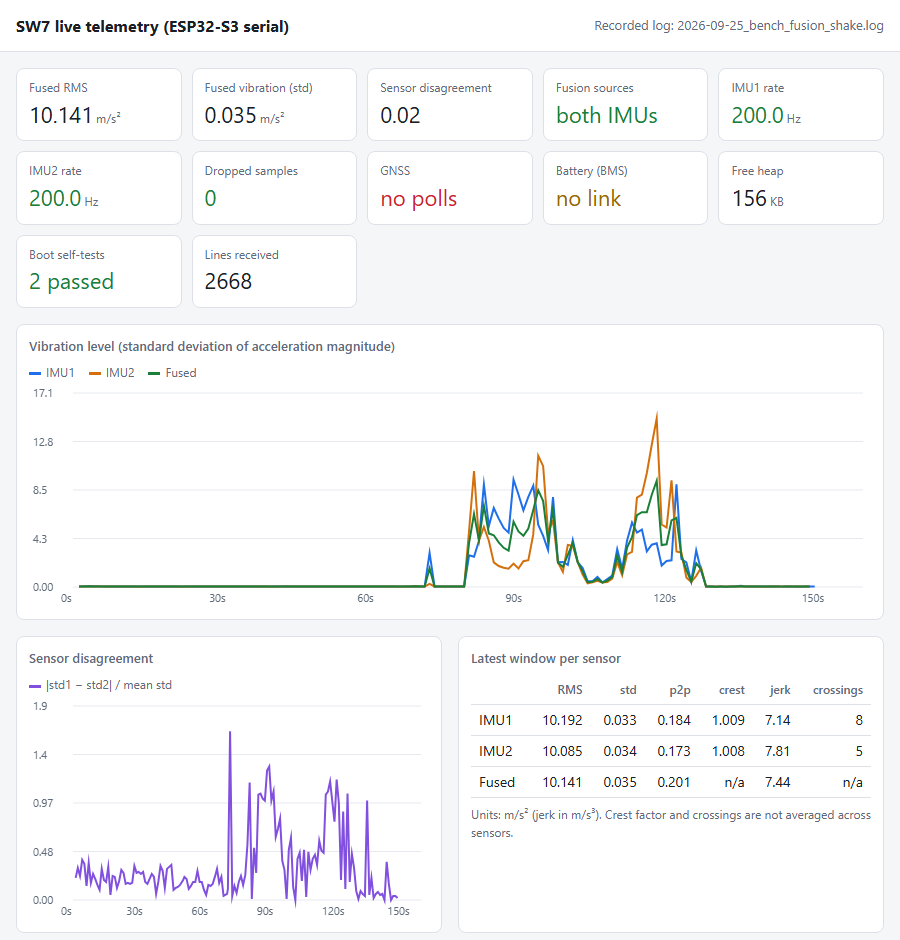
\includegraphics[width=0.8\textwidth]{figures/recorded_session.png}
\caption{A 150-second bench session recorded from power-up and replayed through the dashboard: still until about 75\,s, disturbed by hand until about 128\,s, then still again.}
\label{fig:recorded-session}
\end{figure}

\section{Battery-management system interface over BLE}
\label{sec:bms-interface}

The vehicle's battery pack reports voltage, current, state of charge, capacity, cell and MOSFET temperature, and protection-fault status over a Bluetooth Low Energy interface conforming to the JBD/Jiabaida smart BMS protocol. A prior implementation of this interface existed but had not been integrated into the acquisition architecture described in this chapter, and was found on review to have three defects relevant to a vehicle deployment: it created a new BLE client object on every connection attempt without releasing the previous one, leaking memory at a rate of one client per reconnection cycle; it re-established the BLE connection from scratch every ten seconds regardless of whether the previous connection was still valid, rather than holding a persistent connection; and it framed incoming notification data using only a start byte and a trailing terminator byte, which is unreliable because the terminator's value can legitimately occur inside the data payload itself.

\subsection{Hardened interface design}

The interface was rewritten around a single BLE client object, created once and reused for every connection attempt, with reconnection triggered only by an explicit disconnect callback rather than a fixed timer. Frame reassembly now uses the protocol's declared data-length field (byte index 3) to compute the expected total frame length before attempting to parse a frame, rather than searching for a terminator value that is not guaranteed to be unique. Each frame is additionally validated against a checksum computed as the two's-complement of the sum of the register, status, and length-declared data bytes, following community-documented reverse-engineering of the JBD protocol; a persistent checksum failure is intended as a signal to re-derive this formula from a freshly captured frame rather than as proof the frame itself is corrupt, since no vendor datasheet was available to confirm the formula directly. A secondary plausibility check (pack voltage, state of charge, and current within ranges consistent with a 72\,V nominal pack) is applied independently of the checksum, since a checksum-valid but implausible reading is more likely to indicate a genuine fault condition worth logging than a parsing defect. Every advertised BLE device seen during scanning is logged, not only the configured target address, so that a stale or incorrect address is visible in the log rather than producing silent, unexplained non-connection.

\subsection{A scanning fault found during testing}

During bench testing, the interface was observed to log no BLE advertisements at all, from any device, over an extended scanning window in an environment known to contain multiple active BLE devices. Inspection of the reconnection logic showed that continued scanning had been made conditional on a target-address variable that is only ever set once the target device has already been found, meaning the retry path could never execute on a first run in which the target had not yet been located. Removing that condition, so that scanning resumes whenever the interface is disconnected and not already mid-scan, produced immediate and continuous device discovery on retest. This distinguishes a genuine absence of the target device from a defect preventing the interface from scanning for anything at all, a distinction that would not have been available without the diagnostic logging described above.

\subsection{First live contact with a powered pack}

In a subsequent lab session, the pack was powered on for the first time during testing. The configured MAC address was confirmed present in the scan log, this time carrying an advertised name (\texttt{DB24SA01L24S150ABU}) not seen while the pack was off. Read as a JBD-style model designation, the \texttt{24S} and \texttt{150A} components of this name are consistent with a 24-cell-series lithium pack rated to 150\,A, which is independently useful evidence: it does not match the vehicle's main traction pack, which a separate inherited team's safety documentation records as lead-acid with no BMS. The pack this interface targets is therefore most likely a separate lithium auxiliary pack (plausibly the sensor/accessory supply described by another inherited subsystem's documentation) rather than the vehicle's main battery, a distinction still to be confirmed with that subsystem's owners.

\subsection{A second assumption invalidated by live testing}

With the pack advertising, \texttt{connect()} was observed to succeed on the underlying BLE link, but the subsequent \texttt{getService(BMS\_SERVICE\_UUID)} call returned null, so the connection was dropped before any characteristic was read. This is a second instance of the same class of fault as the scanning defect above: an assumption (that the notify/write characteristics are nested under service UUID \texttt{0xff00}) that had never been tested against a genuinely live pack. It is notable that an independently-written reference implementation, targeting the same MAC address and the same characteristic UUIDs (found in an inherited teammate's codebase), never encounters this problem, because it looks up the notify/write characteristics directly rather than first requiring a specific parent service UUID: a difference in library behaviour (Bleak's high-level API versus this project's direct use of the ESP32 Arduino BLE library) rather than a difference in understanding of the protocol. The interface was corrected to search every service discovered on the connection for the required characteristic UUIDs, rather than assuming which service they belong to, matching the more permissive behaviour of the reference implementation.

Separately, this same cross-check against an independently-written parser confirmed, byte for byte across every decoded field (pack voltage, current, remaining and nominal capacity, protection-fault flags, state of charge, and NTC temperature readings), that this project's own field-offset mapping is correct. This had previously been reverse-engineered from community documentation rather than a vendor datasheet; an independent implementation arriving at identical offsets is meaningful corroborating evidence, though it should be noted that the reference implementation does not itself validate the frame checksum, so the checksum formula specifically remains self-derived and not independently confirmed.

\subsection{Status at time of writing}

After the characteristic-lookup fix, the connection was observed to succeed intermittently rather than reliably: across repeated automatic retry cycles, most \texttt{connect()} attempts failed outright, with one confirmed success (which was the case that exposed the service-UUID fault above). A full power-cycle of the microcontroller did not change this pattern, which rules out a wedged BLE stack on the microcontroller side as the explanation. The pack continued to advertise consistently throughout, which argues against the most likely alternative explanation (another client already holding the pack's single available BLE connection), though this was not conclusively ruled out either. The interface's connection-management and frame-validation logic is therefore now corrected and partially exercised against the real, powered pack, but a fully reliable end-to-end connection, sufficient to capture and checksum-validate a complete real telemetry frame, remains outstanding, and is not yet claimed as complete.

\section{Environmental sensing}
\label{sec:environmental-sensing}

Environmental and air-quality measurement is provided by a Sensirion SEN55 sensor module (part number SEN55-SDN-T), which reports particulate matter, volatile organic compounds (VOC), nitrogen oxides (NOx), relative humidity, and temperature over I\textsuperscript{2}C. The module was selected so that environmental data could be recorded alongside the ride-characterisation and positioning data on the same timeline, allowing conditions along a route to be compared with the vehicle's measured response. It has been ordered from a local supplier; at the time of writing it has not yet been received or integrated into the firmware.

\section{Full-system integration on the target hardware}
\label{sec:full-system-integration}

The work described above (dual-IMU acquisition and calibration, the BMS interface, cellular/GNSS networking) had each been validated individually, but on two different physical boards: the two IMUs on a bare ESP32-S3 development board used for isolated bring-up, and the cellular modem, GNSS, and BMS interface on the project's actual target board (a Makerfabs ESP32-S3 A7670X module, the only board with the required cellular and GNSS hardware present). This section reports moving the IMUs onto the target board itself, so that ride-characterisation, BMS, GNSS, and cellular telemetry publishing all run together on the single physical board the vehicle deployment requires.

\subsection{A misdiagnosed fault: distinguishing a hardware failure from a software configuration mismatch}

After moving the physical IMU connections onto the target board, the firmware produced no serial output whatsoever beyond the ROM bootloader's own boot banner, across repeated reflashes, physical resets, and reseated wiring. Initial hypotheses, tested and each ruled out in turn, included: a hung I2C bus preventing the acquisition task from ever reaching its first diagnostic print (ruled out by adding explicit \texttt{Serial.flush()} calls immediately after \texttt{Serial.begin()}, before any I2C code executes, which still produced no output); insufficient time for native-USB enumeration before the host attempted to read (ruled out by adding a fixed startup delay, which did not change the result); and a damaged connection from the physical rewiring (ruled out by confirming the board's power LED and temperature were normal).

The eventual explanation was a software configuration mismatch rather than a hardware fault. The project's build configuration had, in an earlier session, been changed to route the Arduino \texttt{Serial} object over hardware UART0 rather than native USB, specifically to fix serial output on the bare bring-up board, which reaches the host over UART0 via an external USB-to-serial bridge chip. The target board's own schematic (obtained directly from the manufacturer's public repository, not assumed) shows a materially different design: it exposes three separate USB-C connectors, one wired to the ESP32-S3's native USB peripheral and a second wired to hardware UART0 via an onboard CH340K bridge chip, on an entirely separate physical port from the first. With \texttt{Serial} routed to UART0, application output was being sent out the second, unconnected port, while only the ROM bootloader's fixed-routing boot banner (which uses the native USB peripheral regardless of application configuration) reached the port actually connected to the host. Restoring the native-USB routing configuration for this board resolved the fault immediately and completely.

This is reported in some detail because the debugging process itself is the relevant methodological point: a symptom consistent with several plausible causes (hardware fault, timing issue, software fault) was resolved by systematically eliminating each using a targeted, falsifiable test, rather than assumed from the most recently changed variable. The two boards this project alternates between require opposite settings for this configuration, which is now documented directly in the build configuration file to prevent this specific fault recurring when switching boards again.

\subsection{Result: simultaneous operation on the target hardware}

With the configuration fault resolved, both IMUs, the BMS BLE scanner, and the cellular modem's AT command interface were confirmed running simultaneously on the target board. Both IMUs report as found and configured, each streaming a full window (400-401 samples per 2-second reporting interval, against a 200\,Hz target) with zero dropped samples, and each auto-calibrating on first detection via the procedure described in Section~\ref{sec:imu-magnitude-calibration} (measured scale factors of 1.0390 and 1.0245 for this particular pair of sensors on this board, both stored to non-volatile storage and correctly reloaded on subsequent boots without recalibrating). Concurrently, the modem responded to \texttt{AT+CPIN?} with \texttt{+CPIN: READY}, confirming the SIM is present and unlocked, and logged genuine network-attach events (\texttt{+CGEV: EPS N ACT 1}, \texttt{+CGEV: ME PDN ACT 8}) rather than the modem being silent or erroring, while the BMS scanner continued logging real nearby BLE advertisements throughout. This is the first point at which every major subsystem covered in this chapter has been exercised concurrently on the single physical board the vehicle deployment requires, rather than validated in isolation on separate hardware.

Figure~\ref{fig:bench-setup} shows the bench setup used for this integration, with each component labelled by its role in the system. The Makerfabs board forms the telemetry unit, the Raspberry Pi~4 hosts the camera, and the two are joined by the sync-pulse wire described in Section~\ref{sec:sync-pulse}.

\begin{figure}[htbp]
\centering
\begin{tikzpicture}[
  lbl/.style={font=\footnotesize, text width=3.5cm, inner sep=1pt},
  pin/.style={draw=black, fill=white, circle, inner sep=0pt, minimum size=4.5pt},
  lead/.style={line width=0.6pt, draw=black, preaction={draw=white, line width=2.2pt}}]
\node[anchor=south west, inner sep=0] (img) at (0,0) {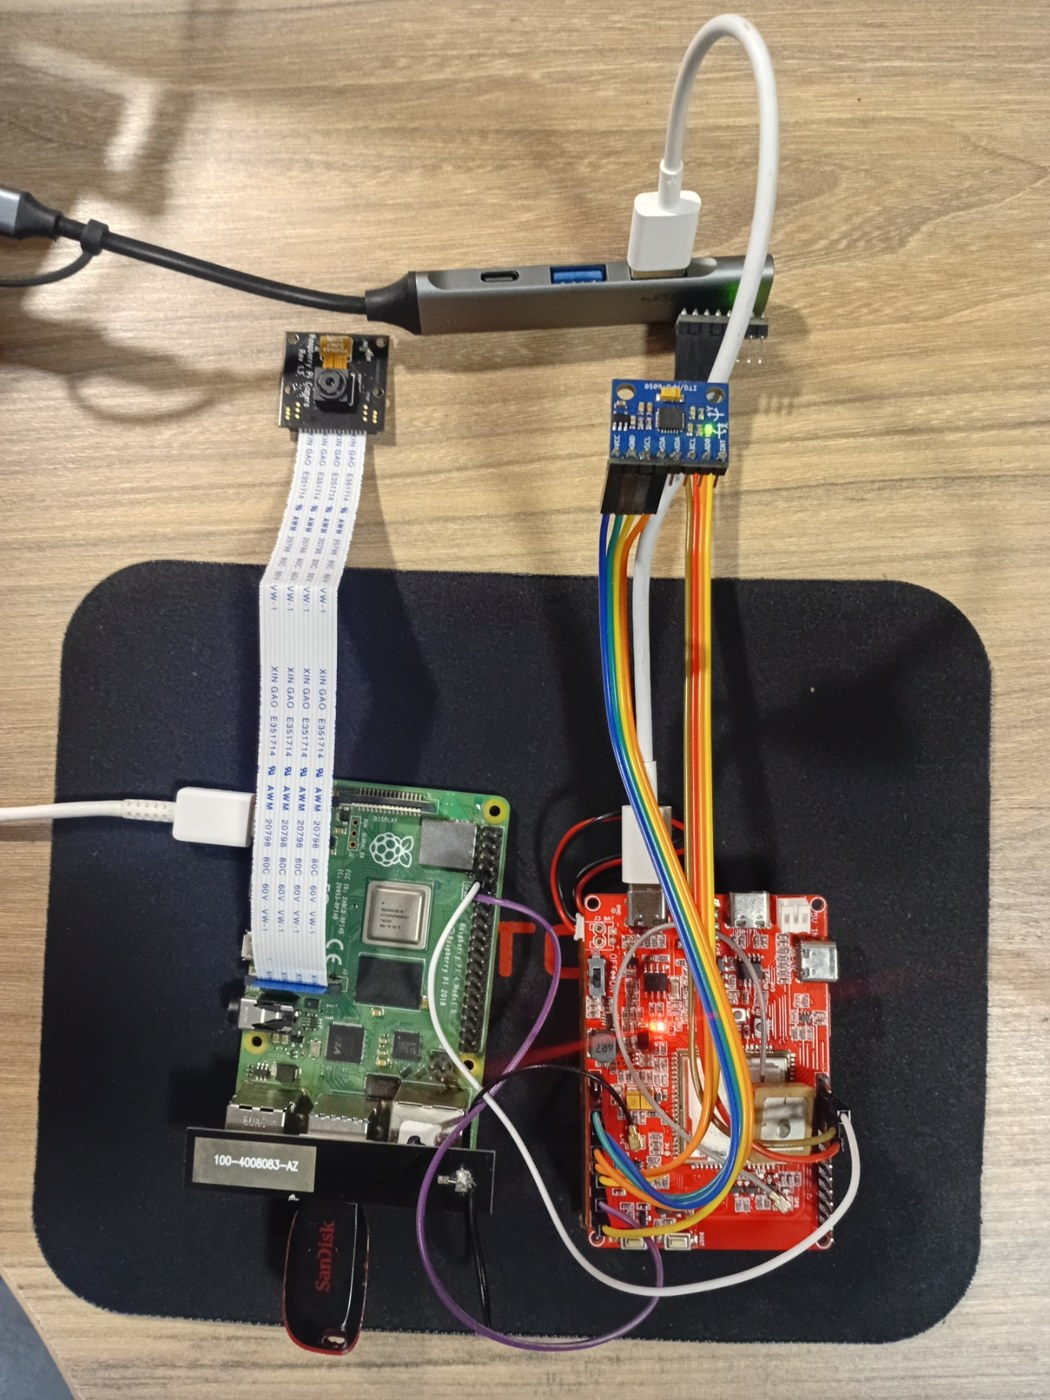
\includegraphics[width=0.5\textwidth]{figures/bench_setup.jpg}};
\begin{scope}[x={(img.south east)}, y={(img.north west)}]
  % left-hand labels
  \node[lbl, anchor=east, align=right] (cam) at (-0.04,0.73) {\textbf{OV5647 camera}\\forward-facing visual record, time-aligned with the IMU data};
  \node[lbl, anchor=east, align=right] (syn) at (-0.04,0.53) {\textbf{Sync-pulse wire}\\ESP32 GPIO to Pi GPIO17, a shared timing reference};
  \node[lbl, anchor=east, align=right] (pi)  at (-0.04,0.35) {\textbf{Raspberry Pi 4}\\camera capture, sync-edge logging and object detection};
  \node[lbl, anchor=east, align=right] (lte) at (-0.04,0.18) {\textbf{LTE antenna}\\for the A7670X cellular modem};
  \node[lbl, anchor=east, align=right] (usb) at (-0.04,0.02) {\textbf{USB drive}\\boot media for the Raspberry Pi};
  % right-hand labels
  \node[lbl, anchor=west, align=left] (hub) at (1.04,0.82) {\textbf{USB hub}\\power and host connection};
  \node[lbl, anchor=west, align=left] (imu) at (1.04,0.64) {\textbf{MPU6050 IMU}\\3-axis acceleration and angular rate, sampled at 200\,Hz};
  \node[lbl, anchor=west, align=left] (esp) at (1.04,0.40) {\textbf{ESP32-S3 and A7670X board}\\IMU acquisition, ride features, BMS over BLE, GNSS, local logging and LTE telemetry};
  \node[lbl, anchor=west, align=left] (gps) at (1.04,0.15) {\textbf{GNSS patch antenna}\\position and speed};
  % leader lines
  \draw[lead] (cam.east) -- (0.32,0.73); \node[pin] at (0.32,0.73) {};
  \draw[lead] (syn.east) -- (0.45,0.37); \node[pin] at (0.45,0.37) {};
  \draw[lead] (pi.east)  -- (0.38,0.28); \node[pin] at (0.38,0.28) {};
  \draw[lead] (lte.east) -- (0.24,0.17); \node[pin] at (0.24,0.17) {};
  \draw[lead] (usb.east) -- (0.31,0.09); \node[pin] at (0.31,0.09) {};
  \draw[lead] (hub.west) -- (0.55,0.79); \node[pin] at (0.55,0.79) {};
  \draw[lead] (imu.west) -- (0.63,0.70); \node[pin] at (0.63,0.70) {};
  \draw[lead] (esp.west) -- (0.66,0.28); \node[pin] at (0.66,0.28) {};
  \draw[lead] (gps.west) -- (0.745,0.20); \node[pin] at (0.745,0.20) {};
\end{scope}
\end{tikzpicture}
\caption{Bench setup of the telemetry system, with each component labelled by its role.}
\label{fig:bench-setup}
\end{figure}

\section{Camera subsystem: Raspberry Pi provisioning and network verification}
\label{sec:pi-camera-provisioning}

A forward-facing camera, intended to provide a synchronised visual record against which inertial events can be labelled (Chapter~\ref{chap:lit}), is hosted on a Raspberry Pi 4 rather than the project's Raspberry Pi 5. This was a deliberate choice: the Raspberry Pi 5 already runs the inherited vehicle dashboard from prior vacation work, and only one storage card was available for the two boards. Provisioning the Raspberry Pi 4 from its own dedicated USB drive, rather than the Raspberry Pi 5's card, avoids modifying or risking a working, inherited deployment in order to develop unrelated capture software.

\subsection{Camera identification}

Querying the connected camera directly (\texttt{rpicam-hello --list-cameras}) identified the sensor as an OV5647, corresponding to the original 5-megapixel Raspberry Pi Camera Module rather than a v2, v3, or High Quality module. This determines the achievable frame rate and resolution combinations available to later experimental work; the sensor supports, among other modes, 1920$\times$1080 at approximately 32.8\,fps and 1296$\times$972 at approximately 46.3\,fps, either of which is adequate for the post-hoc correlation role originally intended for this camera; the later real-time detection role (Section~\ref{sec:hazard-detection}) runs at a lower 640$\times$480 resolution.

\subsection{A media-provisioning fault: incomplete partitioning}

A second Raspberry Pi 4 USB drive, provisioned later to give the camera subsystem its own dedicated boot media independent of the first, was initially written incorrectly: inspecting the resulting drive showed a single FAT32 partition containing only boot files, with no second, larger partition present for the root filesystem. This is consistent with copying the boot-partition files directly onto the drive rather than writing a complete disk image through an imaging tool, since a plain file copy has no means of creating the ext4 root partition the boot configuration expects. The fault was caught by inspecting the drive's partition table directly rather than only its file listing, which showed one partition where two were expected; \texttt{cmdline.txt} on the faulty drive also referenced a root-partition identifier that did not exist anywhere on the disk, which would have caused the device to fail at boot rather than produce a subtler runtime fault. Re-writing the same target drive through Raspberry Pi Imager's normal write flow produced the expected two-partition layout (a $\sim$512\,MB boot partition and a $\sim$29\,GB root partition), which was confirmed both by inspecting the partition table and by cross-checking that the disk's own signature matched the partition identifier referenced in the regenerated \texttt{cmdline.txt}.

\subsection{Network provisioning}

Two network configurations were attempted before a working configuration was found. Joining the existing university network directly was unsuccessful, consistent with existing project documentation noting that the Raspberry Pi 5 is similarly not reachable over the general university network and instead relies on a dedicated mobile hotspot. A local Windows-hosted mobile hotspot was then configured, but the connecting laptop reported that it was sharing the connection over the 5\,GHz band; no device joined the hotspot despite correct network credentials being applied to the Raspberry Pi. This is consistent with a documented characteristic of the Raspberry Pi 4's wireless interface, which requires a wireless regulatory (country) domain to be configured before 5\,GHz operation is enabled at all; without this, the interface cannot use or discover a 5\,GHz-only network, independent of whether the correct credentials are present. Forcing the hotspot to the 2.4\,GHz band resolved this without requiring any change to the Raspberry Pi's own configuration, and the device joined the network immediately following its next reboot.

A related, separate fault was found once the device was network-reachable: the secure-shell service did not respond on its expected port despite the device being fully booted. This was traced to the remote-access configuration not having been re-confirmed during a second provisioning pass that had been intended only to update the wireless network credentials, and was resolved directly on the device (\texttt{systemctl enable --now ssh}). This is noted because it illustrates a general risk in staged device provisioning: revisiting one configuration field to correct it does not guarantee that unrelated fields set in an earlier pass remain applied, and each should be independently verified rather than assumed.

\subsection{A recurring connectivity fault on re-provisioned media}

After the media-provisioning fault above was corrected and the device re-flashed, network connectivity had to be re-established from scratch, and proved considerably less straightforward the second time. The hotspot itself was first found to have stopped broadcasting entirely between sessions (the hosting laptop's virtual network adapter reported a disconnected media state despite appearing enabled in software), which was resolved by re-enabling it directly. With the hotspot broadcasting again, the device still did not detect it. Querying the device's wireless regulatory state directly (\texttt{iw reg get}) showed a discrepancy: the global regulatory domain proposed by the kernel boot parameter correctly showed the expected country code, but the wireless radio itself (\texttt{phy\#0}) reported a separate, generic ``world'' regulatory domain with DFS channels marked unset. This is consistent with a known characteristic of the Broadcom/Cypress wireless chip used on this board, in which the kernel's regulatory-domain hint is not always propagated to the radio's firmware, and a country code set through the driver-level configuration path (via \texttt{raspi-config} or an equivalent wireless-configuration mechanism) is required in addition to the kernel-level hint.

Both the country-code fix and a re-confirmation that the hotspot's own broadcast band was set to 2.4\,GHz (Section~\ref{sec:pi-camera-provisioning} above) were applied together before connectivity was restored, and it is honestly reported here that the specific sufficient fix was not isolated, since testing was not repeated with each change in isolation once a working configuration was found. What is established with confidence is that the device's own radio hardware and driver stack were not blocked by any lower-level fault: \texttt{rfkill} reported no soft or hard block on either the Bluetooth or wireless interfaces throughout, ruling out the simpler explanation that the radio itself was disabled.

\subsection{Verification}
\label{sec:pi-verification}

With network and remote-access issues resolved, the device was confirmed reachable, correctly identified by hostname, running Raspberry Pi OS Trixie (the same release used by the project's Raspberry Pi 5, avoiding a software-version mismatch between the two boards), reporting no under-voltage or thermal throttling condition, and reporting adequate free storage available for recorded video. The combined video-capture and inertial-synchronisation software described in Section~\ref{sec:sync-pulse} was subsequently implemented and validated on this device once connectivity was restored.

A minimal live-preview capability (an MJPEG stream served over HTTP, viewable in any browser without additional software on the viewing machine) was also implemented as an operational aid, allowing the camera's physical aim and framing to be checked remotely before a recording session, independent of the main capture pipeline described above. This capability proved necessary rather than a convenience: without it, a recording session was found only after the fact to have been aimed at the ceiling rather than at any relevant scene, since the camera currently has no fixed mounting bracket and had shifted during handling. The live preview allows this to be caught and corrected before, rather than after, a recording is made, but the underlying cause, the lack of a rigid mount, remains open. The 3D-printed camera casing and corner mount described in Section~\ref{sec:camera-mount} were adopted to address this.

\subsection{Camera casing and mounting}
\label{sec:camera-mount}

Section~\ref{sec:pi-verification} above identifies the absence of a rigid camera mount as an open reliability issue: without one, a recording session was found only after the fact to have been aimed at the ceiling. As a first design, a parametric mounting bracket was modelled in OpenSCAD, sized to the camera module and lens, with a rectangular cable-routing slot and a circular lens aperture. This bracket was not used for the build; the casing that was 3D printed is described below.

An initial render of the design appeared correct in preview, but rendering the full constructive-solid-geometry model (rather than only previewing it) revealed that the cavity cut for the lens aperture extended through the full thickness of the mounting face, consuming the material intended to retain the camera module rather than leaving a lip for it to seat against. This was corrected by bounding the cavity cut height to leave the intended retention lip in place, and re-verified with a full render rather than the preview alone, since the fault was only visible once the model was fully evaluated. Figure~\ref{fig:camera-mount} (Appendix~\ref{app:figures}) shows the corrected design.


The camera is instead housed in a three-part casing designed as part of this project and 3D printed, shown in Figure~\ref{fig:camera-casing} alongside the rest of the bench setup. A bottom shell (29.2 by 28.2 by 7.6\,mm) and a top cover (4.8\,mm) enclose the camera module, protecting it and its ribbon connection, and a separate 30-degree corner mount (32.3\,mm tall) provides the surface by which the casing is attached to the vehicle. A second printed casing houses a second camera. The casing has been printed but not yet fixed to the vehicle, so rigid mounting of the camera remains to be completed during vehicle integration.

\begin{figure}[htbp]
\centering
\begin{tikzpicture}[
  lbl/.style={font=\footnotesize, text width=3.5cm, inner sep=1pt},
  pin/.style={draw=black, fill=white, circle, inner sep=0pt, minimum size=4.5pt},
  lead/.style={line width=0.6pt, draw=black, preaction={draw=white, line width=2.2pt}}]
\node[anchor=south west, inner sep=0] (img) at (0,0) {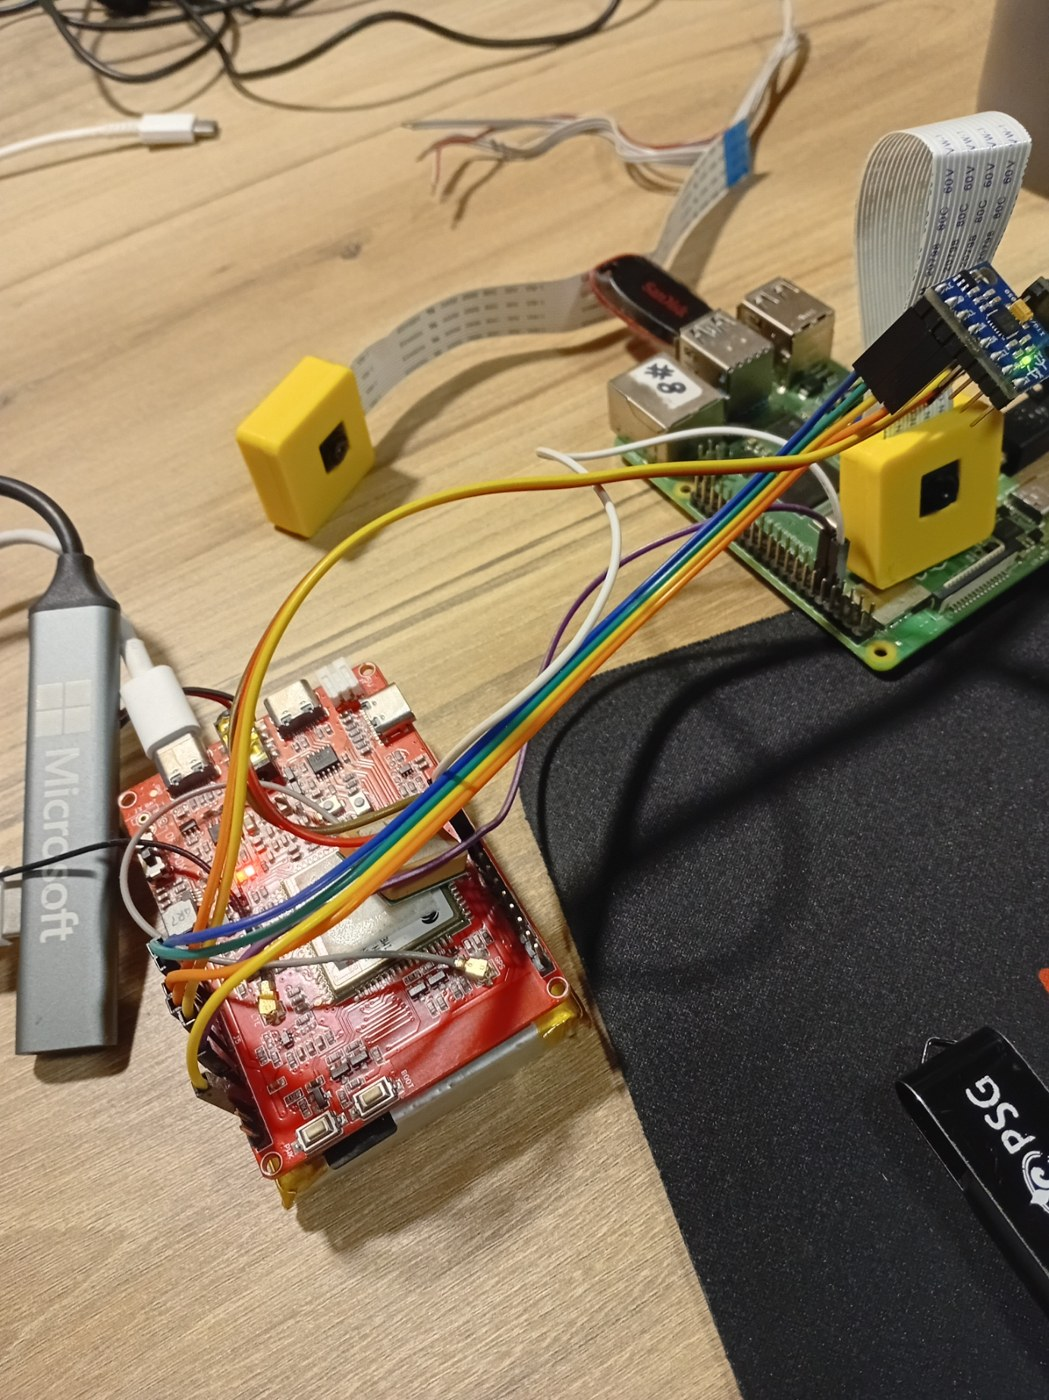
\includegraphics[width=0.5\textwidth]{figures/camera_casing_setup.jpg}};
\begin{scope}[x={(img.south east)}, y={(img.north west)}]
  \node[lbl, anchor=east, align=right] (rib) at (-0.04,0.86) {\textbf{Camera ribbon cable}\\CSI link from the camera to the Raspberry Pi};
  \node[lbl, anchor=east, align=right] (cs1) at (-0.04,0.66) {\textbf{3D-printed camera casing}\\houses and protects the OV5647 camera module};
  \node[lbl, anchor=east, align=right] (esp) at (-0.04,0.30) {\textbf{ESP32-S3 and A7670X board}\\telemetry unit};
  \node[lbl, anchor=west, align=left] (imu) at (1.04,0.88) {\textbf{MPU6050 IMU}\\inertial sensing};
  \node[lbl, anchor=west, align=left] (pi)  at (1.04,0.73) {\textbf{Raspberry Pi 4}\\camera host};
  \node[lbl, anchor=west, align=left] (cs2) at (1.04,0.55) {\textbf{3D-printed camera casing}\\houses the second camera};
  \draw[lead] (rib.east) -- (0.50,0.80); \node[pin] at (0.50,0.80) {};
  \draw[lead] (cs1.east) -- (0.29,0.69); \node[pin] at (0.29,0.69) {};
  \draw[lead] (esp.east) -- (0.33,0.32); \node[pin] at (0.33,0.32) {};
  \draw[lead] (imu.west) -- (0.93,0.79); \node[pin] at (0.93,0.79) {};
  \draw[lead] (pi.west)  -- (0.78,0.75); \node[pin] at (0.78,0.75) {};
  \draw[lead] (cs2.west) -- (0.87,0.64); \node[pin] at (0.87,0.64) {};
\end{scope}
\end{tikzpicture}
\caption{The cameras fitted in their 3D-printed casings, shown with the rest of the bench setup.}
\label{fig:camera-casing}
\end{figure}

\subsection{Hazard-detection scope extension}
\label{sec:hazard-detection}

The camera's role was extended, on supervisor direction, beyond post-hoc visual correlation to include a live hazard-awareness function: reporting the presence, and an estimated rough distance, of road-relevant objects (pedestrians, cyclists, other vehicles) in the camera's field of view. This is deliberately scoped to what the Raspberry Pi 4 can sustain without a dedicated machine-learning accelerator, rather than a full autonomous-driving perception stack: a pretrained, COCO-trained SSD-MobileNet-v1 object detector (quantized to 8-bit integers as a TensorFlow Lite model, requiring no project-specific training data or training run) classifies objects in each frame, and distance is estimated from a known-object-width heuristic using the standard pinhole-camera relationship between an object's real-world width, its width in pixels, and the camera's focal length.

This estimate has two acknowledged limitations, stated here rather than left implicit. First, the focal length used has not yet been calibrated against this specific camera and lens; a placeholder value is used until a calibration shot (an object of known width at a known distance) is captured. Second, each object class uses one fixed average real-world width (for example, 1.8\,m for a car), which is a reasonable order-of-magnitude estimate but not a per-instance measurement, since real vehicles vary in width and are not always presented front-on to the camera. Reported distances should therefore be read as indicative rather than precise until both limitations are addressed.

\subsubsection*{Implementation and data handling}

This component is the only part of the system that uses machine learning: a pretrained, quantised convolutional object-detection network. Its data handling was fixed in code before it first processed live camera frames, on the bench on 28 September 2026.

That data handling is deliberately minimal. The detector reports only a fixed set of object categories (motor vehicles, motorcycles, bicycles, pedestrians, and animals), grouped into coarse distance bands (immediate, warning, and monitoring) rather than precise distances. An object class must be detected within any reportable band for three consecutive frames before an alert is raised, which suppresses single-frame flicker; an active alert is re-logged if the object holds a nearer band for three frames, and clears only after the class has been absent for five consecutive frames. For each alert, only five fields are recorded: object category, distance band, detection confidence, timestamp, and alert status. Each camera frame exists only in memory until the next frame replaces it and is never written to disk. No face or number-plate recognition, and no identification of any individual person or vehicle, is performed. All inference takes place locally on the Raspberry Pi, and the detector has no control over any vehicle function: its output is an advisory alert only. For bench checks, an optional live view draws the detections on the camera image and serves it over the local network; it is not stored.

It is worth stating the boundary clearly in the other direction as well, because the vocabulary invites confusion: the ride-characterisation work described in Section~\ref{sec:ride-characterisation}, including its event detection and classification, is entirely classical time-domain signal processing against hand-set numerical thresholds. It contains no learned parameters and no trained model of any kind.

\subsubsection*{A complementary, non-machine-learning proximity sensor}
\label{sec:tof-sensor}

A separate request arose during this project for a live alert to the driver when an object is near the vehicle, distinct from the post-hoc, camera-based hazard labelling described above. A VL53L5CX time-of-flight sensor (ST Microelectronics) was selected to provide this. It gives a second, physically distinct measurement of nearby objects, involves no camera image or learned model at all, and operates independently of the camera detector, so the alert does not depend on the detector's own status.

Unlike a single-point time-of-flight device, the VL53L5CX resolves distance across an 8$\times$8 grid of independent zones within a 63\textdegree\ diagonal field of view, reporting a distance measurement per zone via I\textsuperscript{2}C at a rated range of up to 4\,m. This was chosen over the narrower single-point VL53L1X specifically for left/centre/right spatial discrimination: a single-point sensor can only report that \emph{something} is ahead within its narrow cone, whereas the zoned output can distinguish which side of the vehicle's path an object occupies. The sensor reports raw per-zone distance only, with no object classification or image capture involved. At the time of writing, the sensor has been sourced (Pololu carrier board, confirmed in stock locally for same-day order) but not yet received or integrated; the alerting logic (a per-zone distance threshold, driving either a GPIO output or a value published alongside the rest of the telemetry described in Section~\ref{sec:mqtt-networking}) is identified as near-term future work once hardware arrives.

The rated 4\,m range and per-zone accuracy are datasheet figures obtained under controlled, indoor lighting. Ambient infrared from direct sunlight is known to reduce the effective range of time-of-flight sensors below their rated figure, and target reflectivity affects the range at which a given object is reliably detected. An independent laboratory characterisation of this exact sensor \cite{caroleo2026} quantifies the reflectivity effect directly rather than leaving it as a general expectation: against a white target, the sensor's reported distance was found to be near-linear with true distance (slope 1.005\,mm/mm) with a standard deviation of only a few millimetres across most of the tested range, whereas against a black target the standard deviation grew to nearly 50\,mm beyond 400\,mm, and the proportion of valid (non-rejected) readings fell to 18.8--34.4\% at the tested distances, against 92--100\% across the study's main experiments. The same study also reports a transient warm-up period of approximately 15 minutes after power-on, during which reported bias drifts as the sensor's internal temperature stabilises. Both effects are expected to be at least as pronounced outdoors on this vehicle, where sunlight adds a further reduction in range beyond what this indoor characterisation captures. This includes dark-coloured road users such as pedestrians in dark clothing, a realistic and safety-relevant case given the finding above, so the sensor's true achievable range and reliability under this project's actual operating conditions is treated as an open question to be measured directly once received, rather than assumed from either the datasheet or this indoor reference study.

\subsubsection*{Why one sensor, not several}

A single-point time-of-flight sensor (such as the VL53L1X considered initially) would need to be duplicated across several fixed pointing directions to give any left/centre/right discrimination, since each unit reports only one aggregate reading for whatever falls within its narrow cone. The VL53L5CX avoids this by construction: it already resolves its 63\textdegree\ field of view into a 8$\times$8 grid of independently reported zones from a single I\textsuperscript{2}C device, so the spatial-discrimination requirement that would otherwise justify multiple sensors is met by one. A second unit would only be justified by a requirement this design does not currently have, such as covering a field of view wider than 63\textdegree\ or sensing in more than one direction from the vehicle (for example, forward and reverse simultaneously); neither is part of the current scope, so one sensor is judged sufficient for this version of the system.

\subsubsection*{Planned bench validation procedure}

Once received, the sensor will be validated on the bench before integration, following the same staged, falsifiable approach used elsewhere in this chapter rather than assumed to work from the datasheet: (1) confirm I\textsuperscript{2}C communication and firmware/driver identification against the expected device ID; (2) reproduce, on this specific unit, the reflectivity-dependent behaviour reported in \cite{caroleo2026} using a plain white and a plain black test target at a fixed known distance, to confirm this unit's own valid-reading rate and bias rather than assuming the published figures transfer directly; (3) sweep a single target through the sensor's rated range at fixed increments to build a measured distance-versus-reported-distance curve, analogous to the self-test already used for the ride-characterisation feature computation (Section~\ref{sec:ride-characterisation}); (4) confirm the per-zone output correctly localises a target moved across the field of view (left, centre, right) rather than only validating the aggregate case; and (5) confirm the warm-up transient reported in \cite{caroleo2026} either is present on this unit or is shown not to materially affect the alert threshold used, before the sensor is relied upon for any on-vehicle test.

\subsubsection*{Status at time of writing}

The detector was first run against the live camera on the bench on 28 September 2026 (Raspberry Pi 4, 640$\times$480 frames, LiteRT runtime), sustaining about 7 frames per second over two 60\,s runs (430 and 419 frames). The first run exposed two input-handling faults. The label file's leading placeholder entry shifted every class name by one, so a person in view was never reported, and the camera's RGB888 buffers are stored in blue, green, red order while the model expects red, green, blue \cite{picamera2manual}. After both were corrected, a person in view was detected with confidence between 0.50 and 0.73; the two fixes were applied together, so their individual effects were not separated. The same run showed an alert clearing on a single missed frame, so one continuously present person produced 16 activations within 47\,s, which led to the clear-side hysteresis described above. Only the person class has so far been confirmed on live frames, distance bands still rely on an uncalibrated focal length, and the detector has not yet been tested outdoors or on the vehicle. A further open question, raised with the project supervisor but not yet answered, is what specifically should count as a reportable hazard for this vehicle and use case (road-surface defects specifically, versus general object presence of any kind); the current implementation reports a fixed set of general COCO object classes as a starting point, pending that clarification.

\subsubsection*{Alert hysteresis}

The alert flicker seen in the second live run came from the clearing rule: an alert cleared on the first frame in which its class was missing, so detections close to the 0.5 confidence threshold switched it off and on repeatedly. The rule was changed so that an active alert clears only after its class has been absent for five consecutive frames, about 0.7\,s at the measured frame rate. An active alert is also logged again if the object holds a nearer distance band for three consecutive frames, the same debounce as an onset, so that an approaching object is recorded as it gets closer while a single noisy frame cannot escalate it. Within a frame, the nearest detection of a class is used, and confidence only decides between detections in the same band. These rules were checked offline, by replaying a scripted sequence of detections through the unchanged detection loop with the camera and model replaced by stand-ins: a person present throughout with single missed frames, a single weak near detection, a sustained approach and a departure. Missed single frames no longer cleared the alert, the single near frame did not escalate it, the sustained approach did, and the alert cleared once the person had gone. The rules have not yet been run against live frames.

\subsubsection*{Live view and latency measurement}

To check that the detector responds to what is actually in front of the camera, and not only through its log, an optional live view was added. It draws each detection (class, confidence, estimated distance and band) on the camera image and serves the result as an MJPEG stream over HTTP, to a browser on the Raspberry Pi itself by default or, when enabled, to other devices on the same local network. Frames exist only in memory and are never written to disk. In the first version the drawing and JPEG encoding ran inside the detection loop, and the detector was then observed to respond more slowly. Drawing and encoding were therefore moved to a separate thread that always takes the newest frame and skips older ones, so a slow viewer delays only the live view and never detection; handing a frame to that thread was measured offline at about 0.3\,ms. The stream also uses a small network send buffer, so a slow link drops frames rather than showing an image that falls further and further behind.

To quantify edge processing latency, as the project brief requires, every frame's latency is now measured from the moment the sensor produced it. Each captured frame carries a \texttt{SensorTimestamp}, which the camera library documents as the time in nanoseconds since boot at which the first pixel was read out of the sensor, on the same clock as the monotonic clock used by the detector \cite{picamera2manual}. The detector records, per frame, the queueing time from readout to capture, preprocessing, inference, and alert logic, and the total from sensor readout to result. It prints the median, 95th percentile and maximum of each every five seconds and can write every frame's timings to a file. The measurement excludes the exposure time itself. Inference also now uses all four processor cores of the Raspberry Pi~4, and the frame is resized with bilinear rather than bicubic interpolation. This instrumentation has been tested offline only; the latency figures on the Raspberry Pi have not yet been measured, and they will set the latency target, including the delay added by the three-frame onset debounce.

\subsubsection*{Alerts feed, dashboard page and start-up service}

So that the vehicle's existing dashboard can show the camera's alerts, the detector also answers a request for its currently active alerts with a short JSON record containing only the five fields of the alert log, plus the current frame rate and latency. A page for the inherited PySide6 dashboard was written that shows the live view and these alerts in the dashboard's own status colours, polls the alerts twice a second, streams video only while the page is on screen, decodes only the newest frame, and reconnects on its own if the camera drops out. It uses only the Qt networking and widget modules, not the web-engine component that has crashed on the dashboard's Raspberry Pi~5. The page was tested offscreen on a laptop inside a copy of the dashboard's code: it picked the newest frame from a stream fed in uneven chunks, listed and cleared alerts, and stayed responsive when the camera address could not be reached. It has not yet been run on the Raspberry Pi~5 or against the live detector, and adding it to the dashboard needs four small edits to the dashboard team's files, which are left for that team to review. A service definition was also written so that the detector starts when the Raspberry Pi~4 boots and restarts if it stops; it has not yet been installed.

\subsubsection*{Colour cast}

In the live view the image looked reddish. Three causes were identified and a test for each written: the channel order in the detector (a blue object should appear blue), the camera itself (comparing with the operating system's own camera preview), and a camera module without an infrared-cut filter, which gives a pink or red cast in daylight and has its own tuning file in the camera software. An option to load that tuning file was added to the detector. The tests have not yet been run, so the cause is not yet known. Because the model was trained on normal-colour images, the cast may also be lowering detection confidence, which the same tests will show by comparing confidence before and after.

A subsequent literature check specifically for camera-based hazard-awareness systems on three-wheeled or auto-rickshaw-class vehicles found no directly comparable academic or open-source system; the closest commercial precedent (a Tier-1 automotive supplier case study describing telematics and HUD products for auto-rickshaws) does not appear to combine camera-based detection with the vehicle-dynamics telemetry described elsewhere in this chapter. This is treated as evidence that the specific integration attempted here is not already a solved problem, rather than as proof of the individual component technologies (pretrained object detection, monocular distance estimation) being novel in themselves, since each of those is independently well precedented in the literature for other vehicle classes.

\section{Cellular telemetry publishing}
\label{sec:mqtt-networking}

A networking task, running inside the existing modem-handling task rather than as a separate FreeRTOS task, publishes a compact JSON summary of the latest ride-characterisation, BMS, and GNSS state over MQTT via the A7670X modem's native AT command set (the same \texttt{AT+CMQTT*} family used by other SIMCom-class modems), rather than requiring a TCP/IP socket library on the microcontroller itself. This was deliberately kept inside the existing modem task rather than given its own task: the modem's UART is not protected by any locking mechanism, and a second task issuing AT commands on the same UART concurrently with the existing GNSS polling would interleave and corrupt both command streams.

The broker address and credentials are left as placeholders in the firmware rather than pointed at the existing Tukzie vac-work team's own Mosquitto broker, whose credentials were deliberately not copied into this project's code. Tested against this placeholder broker, the connect sequence behaved exactly as intended: the AT+CMQTTCONNECT command failed cleanly (confirmed via live serial capture, showing the modem's own error response rather than a silent failure), the failure was logged clearly, and the rest of the system continued operating normally afterward with no crash or hang. This confirmed the AT command sequence itself was implemented correctly, independent of network conditions.

\subsection{Local logging to internal flash}
\label{sec:local-logging}

Telemetry is also recorded locally, so that a session leaves a complete record even with no cellular connection at all. The board's microSD slot was the obvious candidate, but its chip-select line reaches the processor only through a resistor (R23) that the schematic marks as not populated, so there is likely no electrical path to the card as the board is assembled. Rather than build on an interface that may not physically exist, logging uses a LittleFS file system on the processor's own 16\,MB flash, in the 3.5\,MB data partition of the 16\,MB partition table.

Every ten seconds, on the same cadence as MQTT publishing, the complete telemetry record is appended to the log as one JSON line, whether or not the MQTT connection is up; logging is deliberately not conditional on connectivity. The file is capped at 3\,MB, beyond which it is truncated. This first version has two stated limits: truncation discards the oldest data rather than rotating it into a second file, and the log does not yet track which lines have been published, so the unsent backlog is not replayed when the connection returns. The partition mounts correctly on the target board, and its used space grew from 12\,KB to 56\,KB across later boots, consistent with records being written; reading back and checking the logged records has not yet been done.

Enabling the log exposed a side effect on acquisition timing. In the recorded bench session of Section~\ref{sec:imu-fusion}, the longest interval between consecutive samples rose to between 25 and 30\,ms, against a nominal 5\,ms, in one two-second window out of every six, on both IMUs at the same moment, while every other window stayed below 8\,ms. The stalls began about 30 seconds after boot, once the modem's start-up sequence had finished, and then recurred every 12 seconds. Because each GNSS poll currently waits about 3 seconds to time out, the ten-second logging step in the modem loop actually runs every 12 seconds, so the stalls coincide with the flash writes. Writing to flash on the ESP32 briefly suspends code executing from flash on both cores, which would explain both sensors stalling together, although the two are on separate I\textsuperscript{2}C buses. No samples were lost, since the queues absorbed each stall, but the samples around it are unevenly spaced. The link was confirmed on 29 September 2026 with firmware v0.5.0, whose serial console can switch local logging off and on (Section~\ref{sec:mqtt-networking}). With the board still, logging was left on for 120\,s and then switched off for 120\,s, with MQTT publishing every 10\,s throughout. With logging on, both IMUs showed a gap of 33 to 40\,ms every 10\,s, twelve events in the two minutes; with logging off, the longest gap in any window was 5.9\,ms and none exceeded 10\,ms. Both sensors stayed at 200.0 to 200.5\,Hz with no dropped samples in either half. Because publishing continued while logging was off, the stalls come from the flash writes and not from the cellular publish. The stalls now recur every 10\,s rather than 12\,s because the GNSS polls no longer time out in this firmware, so the logging step runs on its nominal cadence (Appendix~\ref{app:evidence}). Candidate remedies are buffering log records in memory and writing them less often, or placing the time-critical acquisition code in instruction RAM; neither has been implemented yet.

\subsection{End-to-end validation against a real broker}

With the full-system integration described in Section~\ref{sec:full-system-integration}, the modem was observed reaching genuine LTE registration: \texttt{AT+CPSI?} returned \texttt{LTE,Online} against a real mobile network operator's PLMN code, and \texttt{AT+CREG?}/\texttt{AT+CGREG?} both reported registered status. This registration was observed to be intermittent across repeated boot sequences in this indoor bench-testing location, in at least one case dropping mid-sequence (\texttt{+CGEV: NW PDN DEACT}) immediately before the MQTT connect attempt, which is reported honestly here as bench-test behaviour rather than smoothed over, since it is directly relevant to how reliably this subsystem could be expected to behave once mounted on the vehicle and moving through areas of varying signal strength.

With the broker address changed from the placeholder to \texttt{test.mosquitto.org} (a public, unauthenticated broker used here only to validate the communication path end-to-end, not as a destination for real vehicle telemetry) and registration present at the time of the attempt, the full sequence succeeded: the firmware logged \texttt{[MQTT] Connected.}, and the subsequent publish returned \texttt{+CMQTTPUB: 0,0}, indicating a successfully acknowledged publish. This is the first point at which a complete, real path (SIM readiness, cellular network registration, PDN context activation, MQTT connection, and message publish) has been exercised end-to-end on real hardware, rather than validated only up to a placeholder failure. The intermittent registration observed above means this should be read as confirmation the mechanism works correctly when network conditions allow it, not as a claim of reliable connectivity under all conditions; the latter would require repeated testing under the vehicle's actual operating conditions, which remains outstanding.

\subsection{Result-code checking and automatic reconnection (firmware v0.5.0)}

A closer reading of the modem manual found a latent fault in the connection code. For the commands that start the MQTT service, connect to the broker and publish, the manual gives both success and failure as an \texttt{OK} followed by a separate result line carrying an error code, where zero means success \cite{simcoma76xx}. The firmware had treated the first \texttt{OK} as success, so it could report a connection that had in fact failed. The acknowledged publish reported above is not affected, since it was confirmed by its own result line (\texttt{+CMQTTPUB: 0,0}). In firmware v0.5.0 these commands wait for their result line and check its code; for the start command, an error response is accepted as meaning the service was already running, as the manual states.

The bench log also showed that after a failed first connection the firmware never tried again. Version 0.5.0 retries with a delay that starts at 30\,s and doubles to at most five minutes, resetting after a success. A session is treated as lost after three failed publishes in a row, or when the modem reports that the server dropped the client or that the network was lost, which the manual says requires the service to be restarted. Before each retry the old session is shut down in the order the manual requires: disconnect, release the client, then stop the service.

Version 0.5.0 also adds commands on the USB serial console for bench and vehicle tests. A line starting with an exclamation mark is handled by the telemetry unit; everything else is still passed straight to the modem. The commands report the state of logging, MQTT and the calibration factors; switch local flash logging off and on, to test whether the periodic acquisition stalls described in Section~\ref{sec:local-logging} come from the flash writes; request an immediate MQTT reconnection; and erase the stored IMU calibration and restart, so that the sensors can be recalibrated in their mounted position without erasing the whole flash. Version 0.5.0 was loaded onto the target board on 29 September 2026 and tested on the bench with a scripted session (\texttt{BenchTest/v050\_bench\_test.py}): the status, logging and reconnect commands all responded; MQTT connected on the first attempt and then published 47 times with no failures; and a requested reconnect shut the session down in the manual's order and reconnected in 0.4\,s. Recovery from a loss of signal was tested on 30 September 2026 by switching the modem's radio off with \texttt{AT+CFUN=4} for 60\,s and back on with \texttt{AT+CFUN=1} (\texttt{BenchTest/signal\_loss\_test.py}). The firmware detected the loss either from the modem's own report, 0.8\,s after the radio went off, or after three failed publishes, 20.7\,s after; it then retried with a delay of 30 and then 60\,s, as designed. In v0.5.0 the reconnect after the radio returned waited for the next scheduled retry and took 36\,s, although the network data connection was back within 2.4\,s. Firmware v0.5.3 therefore also watches for the modem's report that the data connection is active and reconnects within a few seconds of it; in the repeated test it reconnected about 5\,s after the radio came back. In both runs publishing resumed with no failed publishes afterwards. At the start of the repeated test the status showed a live session after two connection attempts, so a failed first connection after boot had been retried successfully; that boot itself was not captured. The recalibration command has not yet been used. When several tasks print at once their serial lines can interleave, which occasionally splits a status line in the log; this affects the readability of logs but not the firmware's behaviour.

\chapter{Results}
\label{chap:results}

This chapter presents the results by subsystem, followed by a full-system test on the vehicle, and maps each back to the research questions and requirements in Table~\ref{tab:requirements-mapping}. Bench-level validation results are reported alongside their methods in Chapter~\ref{chap:method}.

\section{Inertial acquisition integrity (RQ3)}
Achieved sample rate, inter-sample jitter distribution, and dropped-sample counts for both IMUs, first on the bench and then on the moving vehicle.

\section{Sensor calibration}
Per-sensor magnitude calibration factors and the resulting agreement between the two IMUs, at rest and under dynamic excitation.

\section{Ride characterisation (RQ1, RQ4)}
Time-domain features (RMS, peak-to-peak, crest factor, jerk, threshold crossings) and the speed-normalised roughness index recorded over known road sections, compared against identifiable road and powertrain events.

\section{Battery-management telemetry}
BLE connection reliability over a sustained session, and a measured discharge curve compared against the pack's rated capacity.

\section{Camera, synchronisation and proximity sensing}
Camera-to-IMU time alignment, object-detection alert events and the fields recorded for them, and time-of-flight distance measurements, including behaviour against light and dark targets.

\section{Cellular synchronisation and data integrity (RQ3)}
Publish success rate, latency, and recovery behaviour after induced or naturally occurring loss of coverage, with local-log completeness as the reference.

\section{Driver display (RQ2)}
Information hierarchy of the dashboard page as implemented, alert update latency to the screen, legibility under representative lighting, and observed glance time.

\section{Full-system test}
All subsystems operating together on the vehicle over a defined route.

\chapter{Discussion}
\label{chap:discussion}

This chapter interprets the results of Chapter~\ref{chap:results} against the literature of Chapter~\ref{chap:lit} and the research questions. Its main limitation is the one stated throughout: every result is from the bench.

\section{Deterministic acquisition and what it costs}

The synthesis of the literature review noted that edge-telemetry studies are often judged by algorithm accuracy or mean latency, without jitter, queue behaviour or outage recovery (Chapter~\ref{chap:lit}). The results here report those quantities directly: zero dropped samples, the worst gap with and without logging, and the cause of the only recurring gap. The flash-write pause is the clearest example of why they matter. Its rate was cut sixfold by buffering, but its length was not, because the pause comes from the flash itself. A 40\,ms gap in a 200\,Hz stream is eight missing sample instants once a minute, which is small for 1\,s ride windows but would matter for impact detection. Moving logging to separate storage, or to the Raspberry Pi, would be expected to remove it rather than reduce it.

\section{Ride characterisation}

The calibration result supports the review's warning that low-cost inertial measurements depend on the individual sensor: two nominally identical units disagreed by about 8\% at rest, within their datasheet tolerance, and their correction factors changed when they were moved between boards. A ride index that is to be compared across sessions therefore has to be calibrated in its final mounting, which the firmware supports with a single command. The features themselves are computed correctly, but they use the acceleration magnitude rather than a vehicle-fixed vertical axis and have no ISO~2631 frequency weighting, so they describe overall vibration exposure rather than ride comfort as the standard defines it. These are deliberate first-pass simplifications, and both can be added in software once vehicle data exist. The sensors' $\pm8g$ range and 260\,Hz filter are also provisional: the filter lets content between 100 and 260\,Hz alias into the measured band, and the range should be set from the peaks the vehicle actually produces.

RQ4 cannot be answered from the bench. The method is in place: the motor's Hall pulses give its speed, so vibration that tracks motor speed with the vehicle stationary on stands can be separated from vibration that appears only on the road. That separation depends on the Hall tap being wired and on the first vehicle session.

\section{Hazard sensing}

The camera pipeline is fast enough for its purpose: an alert about 0.2\,s after an object appears is about 1.7\,m of travel at 30\,km/h, small against the stopping distance at that speed. The weak point is distance, not speed. The first fused hazard put a person at 0.874\,m by the camera's width heuristic and 0.096\,m by the time-of-flight sensor, so a camera-only distance band could be wrong by a whole band at close range. This is the case for fusion made in Section~\ref{sec:camera-tof-fusion}: the camera says what and in which direction, the sensor says how far. The time-of-flight range of 1.2\,m, however, is only about 0.14\,s of travel at 30\,km/h, so the stand-in sensors serve low-speed manoeuvring and the camera remains the only source at road speed until longer-range sensing is fitted.

The pothole models show the same dependence on local data that the review noted for road-roughness classifiers, whose reported accuracies do not transfer without retraining (Section~\ref{sec:lit-signal-processing}). A model that scored 59.7\% on test images from its own source found almost none of the potholes in South African dashcam footage, and training on tiles cut from the road band of that footage raised the validation score to 0.714. The held-out test score is needed before this improvement can be claimed, and the model has not yet been run on the vehicle's camera, whose view, resolution and colour, without an infrared filter, differ from the dataset's.

\section{Data integrity and connectivity}

Logging independently of the connection, and reconnecting when the modem reports that data are available, gave the store-and-forward behaviour the review identified as necessary for intermittent coverage. The read-back is the important result: it recovered every record, and it found a fault, invalid JSON for missing values, that no amount of watching the live stream had revealed. Two parts of the cellular path remain open: the data go to a public test broker rather than a database, and the backlog of unsent records is not yet replayed after an outage.

\section{Driver display}

The decision to present on the vehicle's existing dashboard rather than a windshield HUD is supported by the review: a head-up position does not by itself make a display safe, its optics are hard to make legible on a removable unit in daylight, and a second display adds a competing channel (Section~\ref{sec:dashboard-page}). Two results bear directly on the safety of what is shown. Live-only mode removes a real hazard found during integration: the dashboard had been showing simulated speed and battery values without any sign when the data link was down. And the touch measurement shows that the panel is not a source of delay, so the lag noticed in bench use comes from the buttons acting on release, which can be changed. What RQ2 asks, whether the display can be read within the 2\,s guidance, has not been measured; the figures for character size, contrast and touch-target size from Chapter~\ref{chap:lit} give a check that can be applied before the on-vehicle observation.

\section{Integration and power}

The most consequential finding of the integration work was not in any one subsystem. The telemetry unit's LTE modem, powered from the Raspberry Pi's USB port, pulled the supply into under-voltage whenever it transmitted, throttled the processor and slowed the detector, and is the likely reason the Raspberry Pi~4 stopped booting on 6 October. The modem worked correctly throughout; the fault was in how the parts were powered together. A separate supply for the telemetry unit is therefore a design requirement for the vehicle installation, not an option.

\section{Validity and limitations}

All results come from one set of hardware on the bench, with the vehicle's vibration, heat, supply and lighting absent. Several parameters are still defaults or uncalibrated: the camera's focal length, the time-of-flight sensor directions, the accelerometer range and filter, and the GNSS speed units. The pothole score is on validation tiles. These limits do not invalidate the bench results, which measure what they claim to measure, but they bound what can be concluded from them, as the next chapter sets out.

\chapter{Conclusions}
\label{chap:conclusions}

This project set out to build a low-cost edge-processing telemetry unit for the TUKZIE Rev 0 electric cargo trike and to present its results safely to the driver. This chapter answers each research question from the evidence in Chapter~\ref{chap:results}, distinguishing what has been shown from what still depends on the vehicle.

\paragraph{RQ1: accuracy and repeatability of the dynamic-response measurement.} The measurement chain is shown to be sound on the bench: two inertial sensors are sampled at a fixed 200\,Hz with no lost samples, including with every other subsystem running; each is calibrated against gravity, which corrects a measured 8\% disagreement between nominally identical units; and the ride features and the dual-sensor fusion are computed correctly. How accurately and repeatably this chain characterises the trike's response to the road and the powertrain has not been measured, because no data have yet been recorded on the moving vehicle. RQ1 is therefore answered for the instrument but not for the vehicle.

\paragraph{RQ2: presenting safety-critical information on the existing dashboard.} A sparse presentation was implemented on the vehicle's own dashboard rather than a second, head-up display: a camera page with the live view and active alerts, a Sensors page with distances and fused hazards, and a banner over every page for an immediate hazard, all showing only live data and marking missing data as absent. On the bench the alerts reach the page within half a second of opening and the touch panel adds no measurable delay. Whether a driver can read this within the 2\,s glance guidance has not been measured, so RQ2 is answered for the information hierarchy and update strategy but not for the driver's glance time.

\paragraph{RQ3: latency, data loss and recovery.} On the bench, acquisition loses no samples; the only recurring pause, from writing the log to flash, is bounded to one 33 to 40\,ms gap a minute; the camera produces a result a median of 102\,ms after the sensor is read; every publish succeeded; the unit reconnects about 5\,s after coverage returns; and the local log is recovered completely. RQ3 is answered for the bench, with the same measures still to be repeated on the moving vehicle.

\paragraph{RQ4: features that separate road from powertrain vibration.} The time-domain features are implemented and verified against a synthetic signal, and the method for separating the two sources, using the motor's Hall pulses as a speed reference, is designed. Without vehicle data and the wired Hall tap, RQ4 is not answered.

\paragraph{Overall.} The project delivers an integrated, low-cost architecture for a three-wheeled electric vehicle: fixed-rate dual-sensor acquisition with measured timing and loss, on-board ride features, camera detection fused with time-of-flight ranging, cellular telemetry with local logging and automatic reconnection (replay of the backlog is not yet implemented), and presentation on the vehicle's existing dashboard. Each part has been measured on the bench, and integrating them exposed faults that no subsystem test showed, the most important being the under-voltage caused by powering the LTE modem from the Raspberry Pi. The work has reached a working bench prototype rather than the demonstration in a relevant environment set as the target in Chapter~\ref{chap:intro}; the on-vehicle sessions, and the calibrations listed in Chapter~\ref{chap:discussion}, are what remain to answer RQ1, RQ2 and RQ4 in full. Recommendations for that work are given in Chapter~\ref{chap:recs}.

\chapter{Recommendations}

\section{Generic road-obstacle detection}

The camera-based detector described in Chapter~3 is restricted to a predefined set of trained object categories (motor vehicles, motorcycles, bicycles, pedestrians, animals). It cannot, and does not claim to, recognise an arbitrary unexpected object, such as fallen debris, that was not one of its training classes; a class like ``stop sign'' would not fire on a twig lying in the road, since the model is a closed-set classifier over its trained categories, not a generic obstacle detector.

Generic detection of this kind is an active, separate research area, referred to in the literature as road-obstacle or road-anomaly detection, distinct from closed-set object detection. HazardNet addresses the scarcity of real hazard training data by augmenting real road images with synthetic 3D debris models under domain randomisation, allowing detection of debris types not explicitly present in training \cite{choe2023hazardnet}. The SegmentMeIfYouCan benchmark provides datasets and an evaluation protocol specifically for anomalous-object and road-obstacle segmentation, that is, identifying objects that do not belong to the expected road scene at all, rather than classifying among a fixed list \cite{chan2021segmentmeifyoucan}. Open-vocabulary detectors such as Grounding DINO, which pair a Transformer-based detector with language-grounded pre-training to detect objects described by an arbitrary text prompt rather than a fixed class list \cite{liu2023groundingdino}, offer an alternative route, but as large Transformer-based models they are unlikely to run in real time on a Raspberry Pi 4 without a hardware accelerator, which would need to be confirmed by measurement. A more Pi-appropriate direction is a lightweight, custom-trained detector: a 2026 study demonstrates a YOLOv8-n model trained specifically on rare roadside obstacles (cones, debris, barrels, fallen trees, rocks), reporting 98.1\% mAP@0.5 at 68\,fps on GPU hardware \cite{tanveer2026yolov8n}, though this would need re-validation for real-time performance on the Pi 4's more limited compute.

None of these approaches is recommended for adoption within the current project. Each would replace the detection model already implemented, and would require its own dataset, training, and on-hardware evaluation before it could be trusted. Generic road-obstacle detection is therefore recorded here as a concrete, evidenced direction for future work, rather than attempted within the scope or timeline of this dissertation.

Were this pursued in a subsequent project phase, a sensible order of work would be: define the operational meaning of ``unexpected obstacle'' for this vehicle and use case; collect and annotate representative road-hazard imagery, or evaluate an existing benchmark such as RoadObstacle21; compare a custom lightweight detector against an anomaly-segmentation approach on that data; test detection accuracy across daylight, night, rain, shadow, and glare conditions, since the present system has only been characterised under bench lighting; measure inference speed and power draw on the actual Raspberry Pi 4 rather than the GPU hardware the cited studies were evaluated on; calibrate any resulting distance estimate against the VL53L5CX time-of-flight sensor described in Section~\ref{sec:tof-sensor} as an independent reference, rather than trusting a vision-only estimate alone; and only then begin live-camera testing of the new model.

% IEEE numbered reference style.
% With thebibliography, the printed number of an entry is its POSITION in this list.
% Entries are in order of first citation, and uncited entries were removed (10 Oct 2026).
% A new source goes where it is first cited; the text uses \cite, so numbers update.

\begin{thebibliography}{99}
\bibitem{unwup2019} United Nations, Department of Economic and Social Affairs, Population Division, \emph{World Urbanization Prospects: The 2018 Revision}. New York, NY, USA: United Nations, 2019.

\bibitem{sebwa2025} O. S. Sebwa, P. V. Chombo, G. B. Gerutu, R. O. Kivugo, J. H. Hosea, and K. A. Greyson, ``Energy, economy and environmental assessment of e-tricycle for medium-size cargo deliveries: A case of Dar es Salaam City,'' \emph{The Journal of Engineering}, vol. 2025, no. 1, Art. no. e70073, 2025, doi: 10.1049/tje2.70073.

\bibitem{who2023} World Health Organization, \emph{Global Status Report on Road Safety 2023: Summary}. Geneva, Switzerland: World Health Organization, 2023.

\bibitem{liu2003} Y.-C. Liu, ``Effects of using head-up display in automobile context on attention demand and driving performance,'' \emph{Displays}, vol. 24, nos. 4--5, pp. 157--165, 2003, doi: 10.1016/j.displa.2004.01.001.

\bibitem{hauslschmid2015} R. H\"auslschmid, S. Osterwald, M. Lang, and A. Butz, ``Augmenting the driver's view with peripheral information on a windshield display,'' in \emph{Proc. 20th Int. Conf. Intelligent User Interfaces}, 2015, doi: 10.1145/2678025.2701393.

\bibitem{nhtsa2013} National Highway Traffic Safety Administration, \emph{Visual-Manual NHTSA Driver Distraction Guidelines for In-Vehicle Electronic Devices}, Federal Register, vol. 78, no. 81, pp. 24818--24890, Apr. 2013.

\bibitem{barnell2018} M. Barnell, C. Raymond, C. Capraro, D. Isereau, C. Cicotta, and N. Stokes, ``High-performance computing (HPC) and machine learning demonstrated in flight using Agile Condor,'' in \emph{Proc. IEEE High Performance Extreme Computing Conf.}, 2018, pp. 1--4, doi: 10.1109/HPEC.2018.8547797.

\bibitem{mareska2022} A. Mare\v ska, T. Kordov\'a, and M. Havl\'ik M\'ika, ``Production of Head-Up Display windshield and its relation with the image quality,'' \emph{Transactions on Transport Sciences}, vol. 13, no. 2, pp. 63--70, 2022, doi: 10.5507/tots.2022.011.

\bibitem{canomarin2016} E. Ca\~no-Mar\'in, P. E. Gonz\'alez Prieto, M. Maroto G\'omez, and D. Villegas, ``Head-up displays in driving,'' 2016, arXiv:1803.08383.

\bibitem{zhu2021} Y. Zhu, Y. Jing, M. Jiang, Z. Zhang, D. Wang, and W. Liu, ``An experimental study of the cognitive load of in-vehicle multiscreen connected HUD,'' in \emph{Design, User Experience, and Usability: Design for Contemporary Technological Environments}, Lecture Notes in Computer Science, vol. 12781. Cham, Switzerland: Springer, 2021, pp. 268--285, doi: 10.1007/978-3-030-78227-6\_20.

\bibitem{kimmel2020} W. M. Kimmel, C. D. Weiss, and A. M. Mazzuchi, \emph{Technology Readiness Assessment Best Practices Guide}, NASA/SP-20205003605, 2020.

\bibitem{fhwa2016} Federal Highway Administration, \emph{Measuring and Specifying Pavement Smoothness}, Tech. Brief FHWA-HIF-16-032, Washington, DC, USA, 2016.

\bibitem{alatoom2025} Y. I. Alatoom and O. Smadi, ``Embedded framework for low-cost pavement condition evaluation using microcontroller and single-board computer platforms,'' \emph{Automation in Construction}, vol. 178, Art. no. 106442, 2025, doi: 10.1016/j.autcon.2025.106442.

\bibitem{winberg2026} S. Winberg and S. Jayalath, ``Development of an Embedded HPEC Telemetry Unit and Windshield HUD for the TUKZIE Rev 0 Platform,'' EEE4022S project brief, University of Cape Town, Department of Electrical Engineering, 2026.

\bibitem{jinpengmanual} Jiangsu Jinpeng Group Co., Ltd, \emph{Electric Tricycle User Manual}. Vehicle documentation, TUKZIE Rev 0 platform.

\bibitem{adamsrasara2026} N. Adams and S. Rasara, ``Jinpeng Electric Tricycle Drivetrain: Characterization \& Modelling,'' TUKZIE vacation work report, University of Cape Town, Department of Electrical Engineering, Jul. 2026.

% Verified 2026-09-24 via Crossref and Semantic Scholar abstract: uses mean
% square of unsprung-mass acceleration divided by vehicle speed.

\bibitem{bui2026} V.-H. Bui, D.-N. Tran, P. Q. Huy, N. V. Cong, and T.-H. Dao, ``Signal processing-driven real-time rough road detection with GPS accuracy improvement on edge microcontrollers,'' in \emph{Proc. IEEE 15th Int. Conf. Communication Systems and Network Technologies}, 2026, doi: 10.1109/CSNT69054.2026.11502079.

\bibitem{hauslschmid2016} R. H\"auslschmid, B. Pfleging, F. Alt, and A. Butz, ``A design space to support the development of windshield applications for the car,'' in \emph{Proc. 2016 CHI Conf. Human Factors in Computing Systems}, 2016, pp. 5076--5091, doi: 10.1145/2858036.2858336.

\bibitem{saenz2016} J. Saenz, M. Figliozzi, and J. Faulin, ``Assessment of the carbon footprint reductions of tricycle logistics services,'' \emph{Transportation Research Record}, vol. 2570, no. 1, pp. 48--56, 2016, doi: 10.3141/2570-06.

\bibitem{gonzalez2008} A. Gonz\'alez, E. J. O'Brien, Y.-Y. Li, and K. Cashell, ``The use of vehicle acceleration measurements to estimate road roughness,'' \emph{Vehicle System Dynamics}, vol. 46, no. 6, pp. 483--499, 2008, doi: 10.1080/00423110701485050.

\bibitem{sattar2018} S. Sattar, S. Li, and M. Chapman, ``Road surface monitoring using smartphone sensors: A review,'' \emph{Sensors}, vol. 18, no. 11, Art. no. 3845, 2018, doi: 10.3390/s18113845.

\bibitem{yiliguoqi2026} B. Yiliguoqi, B. Siriguleng, Arong, G. Guo, and J. Wang, ``Research on the evaluation and analysis of road surface roughness based on smartphone sensors and SVM,'' \emph{Scientific Reports}, vol. 16, Art. no. 4409, 2026, doi: 10.1038/s41598-025-34396-3.

\bibitem{iso2631} International Organization for Standardization, \emph{Mechanical Vibration and Shock: Evaluation of Human Exposure to Whole-Body Vibration, Part 1: General Requirements}, ISO 2631-1:1997, including Amendment 1:2010.

\bibitem{shi2016} W. Shi, J. Cao, Q. Zhang, Y. Li, and L. Xu, ``Edge computing: Vision and challenges,'' \emph{IEEE Internet of Things Journal}, vol. 3, no. 5, pp. 637--646, 2016, doi: 10.1109/JIOT.2016.2579198.

\bibitem{perezgonzalez2025} A. P\'erez-Gonz\'alez, A. F. Villa-Salazar, I. N. Gomez-Miranda, J. D. Vel\'asquez-G\'omez, A. F. Romero-Maya, and A. Jaramillo-Duque, ``An IoV-based real-time telemetry and monitoring system for electric racing vehicles: Design, implementation, and field validation,'' \emph{Vehicles}, vol. 7, no. 4, Art. no. 128, 2025, doi: 10.3390/vehicles7040128.

\bibitem{smith2016} M. Smith, J. L. Gabbard, and C. Conley, ``Head-up vs. head-down displays: Examining traditional methods of display assessment while driving,'' in \emph{Proc. 8th Int. Conf. Automotive User Interfaces and Interactive Vehicular Applications}, 2016, pp. 185--192, doi: 10.1145/3003715.3005419.

\bibitem{reimer2014typeface} B. Reimer, B. Mehler, J. Dobres, J. F. Coughlin, S. Matteson, D. Gould, N. Chahine, and V. Levantovsky, ``Assessing the impact of typeface design in a text-rich automotive user interface,'' \emph{Ergonomics}, vol. 57, no. 11, pp. 1643--1658, 2014, doi: 10.1080/00140139.2014.940000.

\bibitem{you2021charsize} F. You, Y.-F. Yang, M.-T. Fu, J. Zhang, and J.-M. Wang, ``Design guidelines for the size and length of Chinese characters displayed in the intelligent vehicle's central console interface,'' \emph{Information}, vol. 12, no. 5, p. 213, 2021, doi: 10.3390/info12050213.

\bibitem{kim2014touchkey} H. Kim, S. Kwon, J. Heo, H. Lee, and M. K. Chung, ``The effect of touch-key size on the usability of in-vehicle information systems and driving safety during simulated driving,'' \emph{Applied Ergonomics}, vol. 45, no. 3, pp. 379--388, 2014, doi: 10.1016/j.apergo.2013.05.006.

\bibitem{euroncap2026engagement} Euro NCAP, \emph{Safe Driving: Driver Engagement Protocol}, version 1.2. Leuven, Belgium: Euro NCAP, 2026.

\bibitem{strayer2017infotainment} D. L. Strayer, J. M. Cooper, R. M. Goethe, M. M. McCarty, D. J. Getty, and F. Biondi, \emph{Visual and Cognitive Demands of Using In-Vehicle Infotainment Systems}. Washington, DC, USA: AAA Foundation for Traffic Safety, 2017.

\bibitem{currano2021} R. Currano, S. Y. Park, D. J. Moore, K. Lyons, and D. Sirkin, ``Little Road Driving HUD: Heads-Up Display complexity influences drivers' perceptions of automated vehicles,'' in \emph{Proc. 2021 CHI Conf. Human Factors in Computing Systems}, 2021, pp. 1--15, doi: 10.1145/3411764.3445575.

% CORRECTED 04 Sep 2026: this entry previously cited "SA Motorcycles" as
% the vehicle manufacturer. Three independent sources - the drivetrain
% team's nameplate reading (see adamsrasara2026 below), the Tukzie
% dashboard's own simulation constants, and this vehicle's own user
% manual - all identify the platform as a Jinpeng, not an SA Motorcycles
% product. The entry below cites that manual directly.

\bibitem{park2020} K. Park and Y. Im, ``Ergonomic guidelines of Head-Up Display user interface during semi-automated driving,'' \emph{Electronics}, vol. 9, no. 4, Art. no. 611, 2020, doi: 10.3390/electronics9040611.

\bibitem{qin2017} Z. Qin, F.-C. Lin, Y.-P. Huang, and H.-P. D. Shieh, ``Maximal acceptable ghost images for designing a legible windshield-type vehicle Head-Up Display,'' \emph{IEEE Photonics Journal}, vol. 9, no. 6, pp. 1--12, 2017, doi: 10.1109/JPHOT.2017.2758820.

\bibitem{desimone2018} M. De Simone, Z. B. Rivera Chavez, and D. Guida, ``Obstacle Avoidance System for Unmanned Ground Vehicles by Using Ultrasonic Sensors,'' \emph{Machines}, vol. 6, no. 2, Art. no. 18, 2018, doi: 10.3390/machines6020018.

\bibitem{noomwongs2025} N. Noomwongs, K. Kiataramgul, S. Chantranuwathana, and G. Phanomchoeng, ``GNSS-RTK-Based Navigation with Real-Time Obstacle Avoidance for Low-Speed Micro Electric Vehicles,'' \emph{Machines}, vol. 13, no. 6, Art. no. 471, 2025, doi: 10.3390/machines13060471.

% NEW - added for Recommendations, future work on generic road-obstacle
% detection (distinct from the closed-set detector actually implemented).

\bibitem{caroleo2026} G. Caroleo, A. Albini, and P. Maiolino, ``On the Characterisation of the Time-of-Flight VL53L5CX Sensor by STMicroelectronics for Indoor Robotics Applications,'' \emph{Sensors}, vol. 26, no. 5, Art. no. 1639, 2026, doi: 10.3390/s26051639.

\bibitem{makerfabsa7670x} Makerfabs, ``ESP32S3 4G LTE CAT1 A7670X,'' product page and hardware repository. [Online]. Available: \url{https://www.makerfabs.com/esp32s3-4g-lte.html} and \url{https://github.com/Makerfabs/ESP32-S3-4G-LTE-CAT1-A7670X} (accessed 24 Sep. 2026).

% Verified 2026-09-24: genuine 652-page manual, documents every AT command
% used in Ch.3. Its +CGNSSINFO format (16 fields) does NOT match the 9-field
% response the fitted modem returned, so this is the version consulted, not
% confirmed as the version matching the module's firmware (see Ch.3 GNSS).

\bibitem{simcoma76xx} SIMCom Wireless Solutions, \emph{A76XX Series AT Command Manual}, V1.09, Apr. 2023. [Online]. Available: \url{https://files.waveshare.com/wiki/A7670E-Cat-1-GNSS-HAT/A76XX_Series_AT_Command_Manual_V1.09.pdf} (accessed 24 Sep. 2026).

% Verified 2026-09-28: manual build dated 2026-09-15, p. 21 "Image Formats":
% "RGB888 - 24 bits per pixel, ordered [B, G, R]."

\bibitem{li2018} Z. Li, W. Yu, and X. Cui, ``Online Classification of Road Roughness Conditions with Vehicle Unsprung Mass Acceleration by Sliding Time Window,'' \emph{Shock and Vibration}, vol. 2018, Art. no. 5131434, 2018, doi: 10.1155/2018/5131434.

% NEW - added for the VL53L5CX proximity-alerting subsection (Methodology,
% Section on non-ML alternatives). Open-access; confirmed via PMC/MDPI.

\bibitem{sensirionsen5x} Sensirion AG, \emph{Datasheet SEN5x: Environmental Sensor Node for HVAC and Air Quality Applications}, version 2, Stäfa, Switzerland, Mar. 2022.

\bibitem{picamera2manual} Raspberry Pi Ltd, \emph{The Picamera2 Library}, Sep. 2026. [Online]. Available: \url{https://datasheets.raspberrypi.com/camera/picamera2-manual.pdf} (accessed 28 Sep. 2026).

% NEW - added for the vehicle-identity correction above (Introduction, Scope).

\bibitem{choe2023hazardnet} T. E. Choe, J. Wu, X. Lin, K. Kwon, and M. Park, ``HazardNet: Road Debris Detection by Augmentation of Synthetic Models,'' arXiv:2303.07547, 2023.

\bibitem{chan2021segmentmeifyoucan} R. Chan, K. Lis, S. Uhlemeyer, H. Blum, S. Honari, R. Siegwart, P. Fua, M. Salzmann, and M. Rottmann, ``SegmentMeIfYouCan: A Benchmark for Anomaly Segmentation,'' in \emph{Proc. Neural Information Processing Systems (NeurIPS) Track on Datasets and Benchmarks}, 2021.

\bibitem{liu2023groundingdino} S. Liu, Z. Zeng, T. Ren, F. Li, H. Zhang, J. Yang, Q. Jiang, C. Li, J. Yang, H. Su, J. Zhu, and L. Zhang, ``Grounding DINO: Marrying DINO with Grounded Pre-Training for Open-Set Object Detection,'' arXiv:2303.05499, 2023.

\bibitem{tanveer2026yolov8n} A. Bint-e Tanveer, M. A. Kamal, M. M. Alam, and M. Mohd Su'ud, ``Real-time detection of rare roadside obstacles using YOLOv8-n in autonomous vehicles,'' \emph{PLOS ONE}, 2026, doi: 10.1371/journal.pone.0350732.

\bibitem{raspberrypigpio} Raspberry Pi Ltd, ``Raspberry Pi hardware: GPIO and the 40-pin header,'' Raspberry Pi documentation. [Online]. Available: \url{https://www.raspberrypi.com/documentation/computers/raspberry-pi.html}

\end{thebibliography}

\appendix
\chapter{Graduate Attributes, AI Use and Project Repository}

\section{Graduate attribute evidence}

\begin{longtable}{||p{2em} |p{9em} |p{22em}||}
 \hline
 \textbf{GA} & \textbf{Requirement} & \textbf{Justification and section in the report}  \\ [0.5ex]
 \hline\hline
 \endhead
 1 & Problem-solving & Research questions framed around measurable dynamic response (Section~\ref{sec:requirements-mapping}); faults root-caused from first principles, including the speed dependence of raw RMS (Section~\ref{sec:speed-norm}) and the Serial-routing fault (Section~\ref{sec:full-system-integration}). \\
 \hline
 4 & Investigations, experiments and data analysis & Hypothesis-test-conclusion investigations of the GNSS format (Section~\ref{sec:gnss-parsing-validation}) and BMS protocol (Section~\ref{sec:bms-interface}); synthetic-signal validation and per-sensor calibration (Section~\ref{sec:imu-magnitude-calibration}); camera-to-IMU timing bounds (Section~\ref{sec:sync-pulse}). \\
 \hline
 5 & Use of engineering tools & PlatformIO, FreeRTOS and serial diagnostics (Chapter~3); staged flash and PSRAM configuration testing (Section~\ref{sec:flash-psram}); OpenSCAD bracket design and the 3D-printed camera casing (Section~\ref{sec:camera-mount}). \\
 \hline
 6 & Professional and technical communication (Long report) & This report. \\
 \hline
 8 & Individual work & Independent design decisions, including sensor selection (Section~\ref{sec:tof-sensor}) and the data handling designed into the object detector (Section~\ref{sec:hazard-detection}). \\
 \hline
 9 & Independent learning ability & Self-corrected assumptions against primary sources (schematics, live tests); literature-driven narrowing of the research gap (Chapter~2). \\ [1ex]
 \hline
\end{longtable}

\section{Project repository}

Firmware, camera software, planning documents and supporting tools for this project are available at \url{https://github.com/0geder/Tukzie-HPEC-HUD}.

\section{Declaration of Artificial Intelligence Use}

Artificial intelligence tools were used to assist with clarifying the organisation of this report, improving the alignment and consistency of its presentation, refining wording, and checking LaTeX formatting. All AI-assisted suggestions were reviewed by the author. The author remains responsible for the report's technical content, analysis, interpretations, and final editorial decisions.


\chapter{Supporting Figures}
\label{app:figures}

The figures below support the text of Chapters~1 and~3, where each is referenced.

\begin{figure}[htbp]
\centering
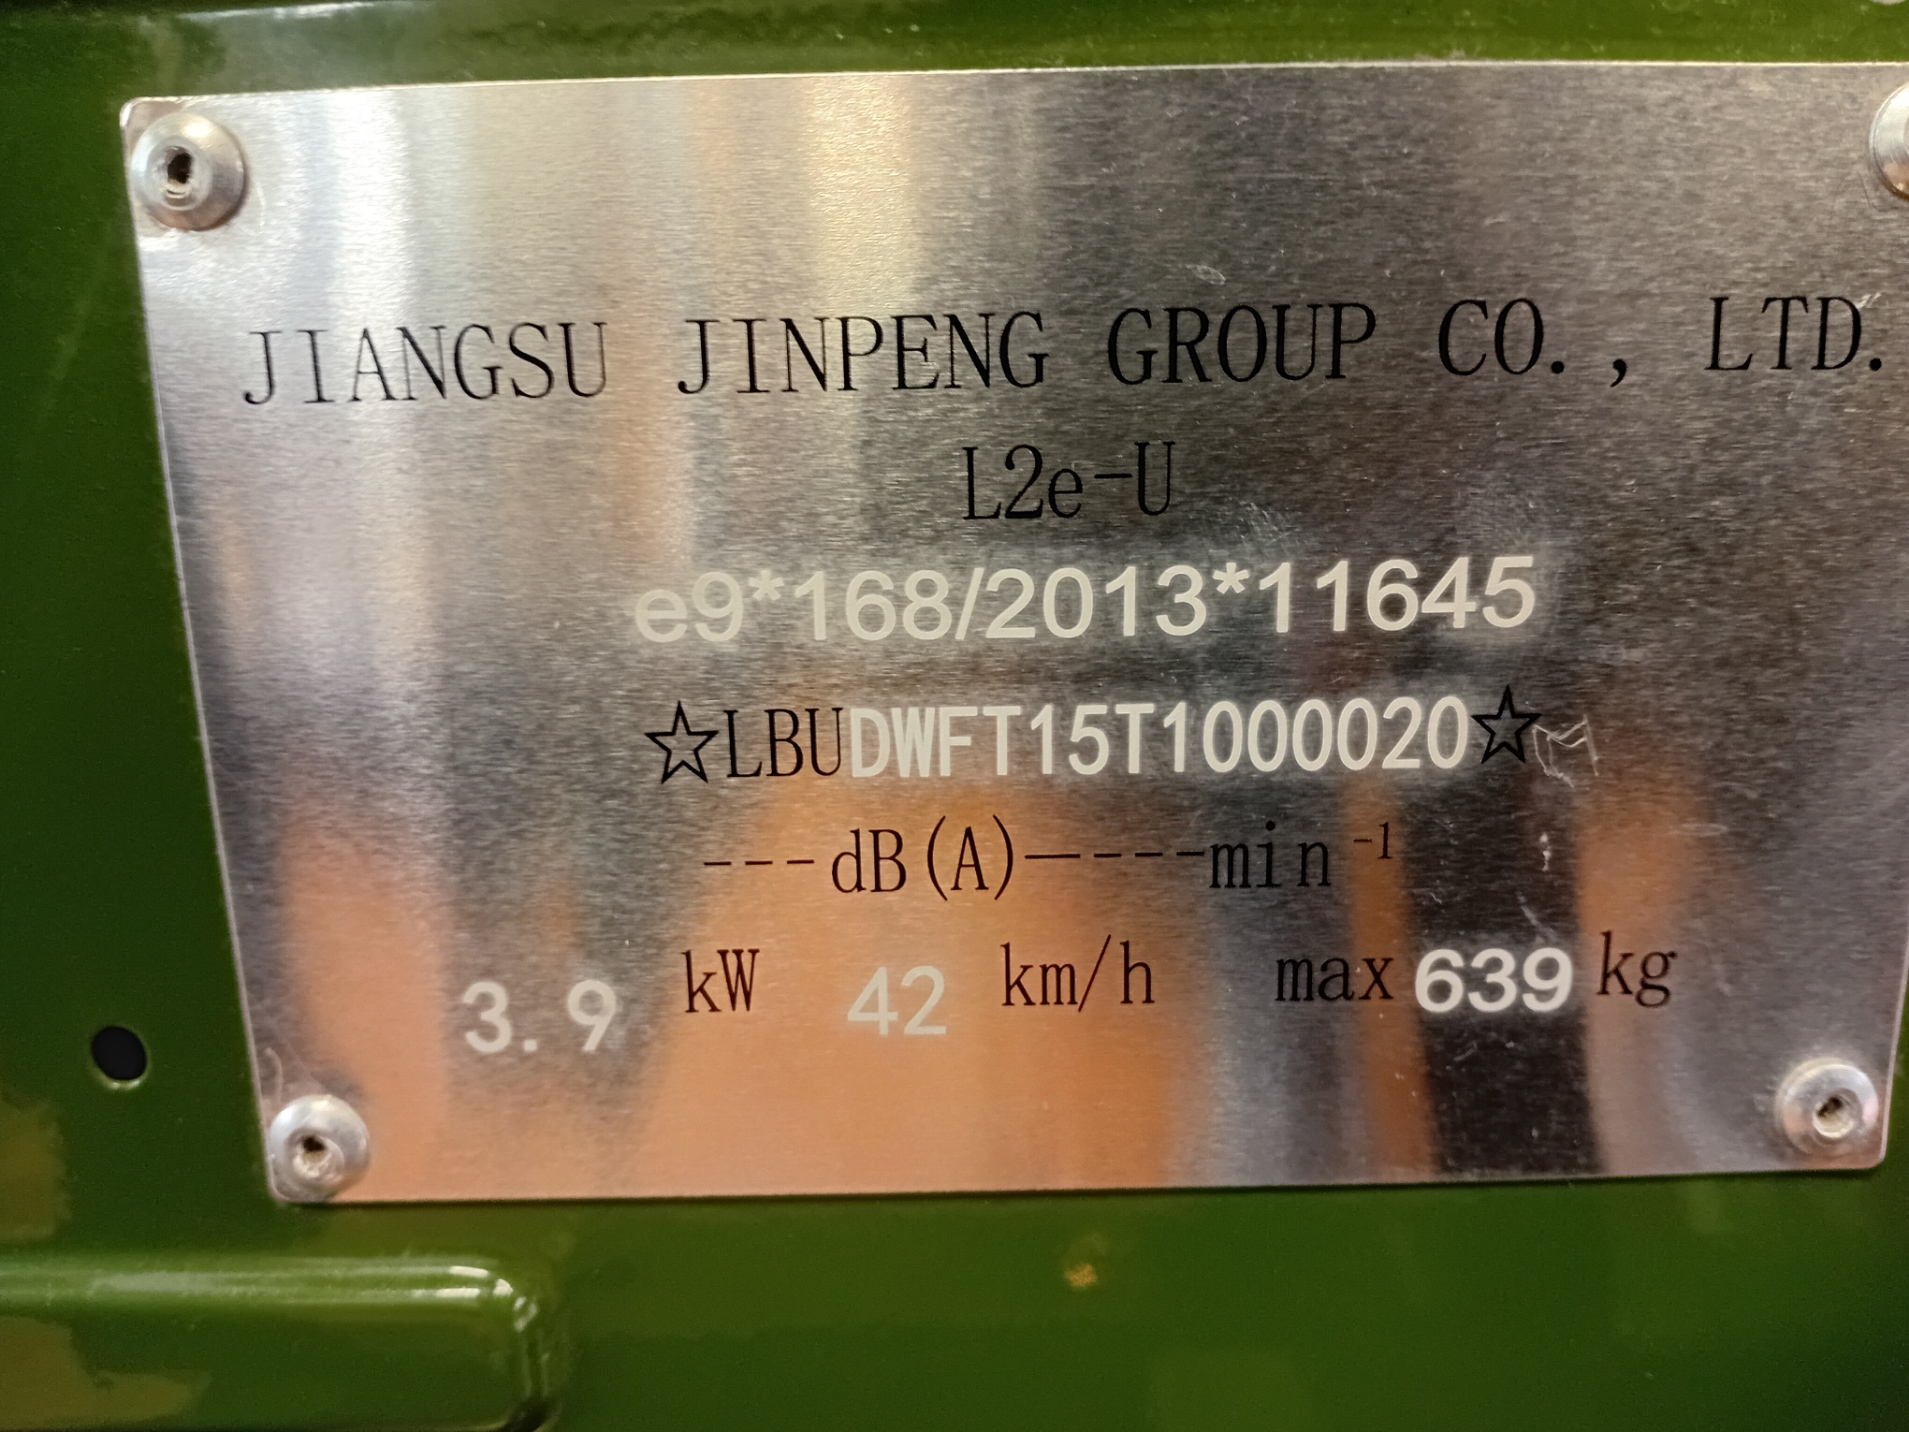
\includegraphics[width=0.55\textwidth]{figures/vehicle_nameplate.jpg}
\caption{Manufacturer identification plate on the TUKZIE Rev 0 platform, photographed directly during vehicle inspection.}
\label{fig:vehicle-nameplate}
\end{figure}

\begin{figure}[htbp]
\centering
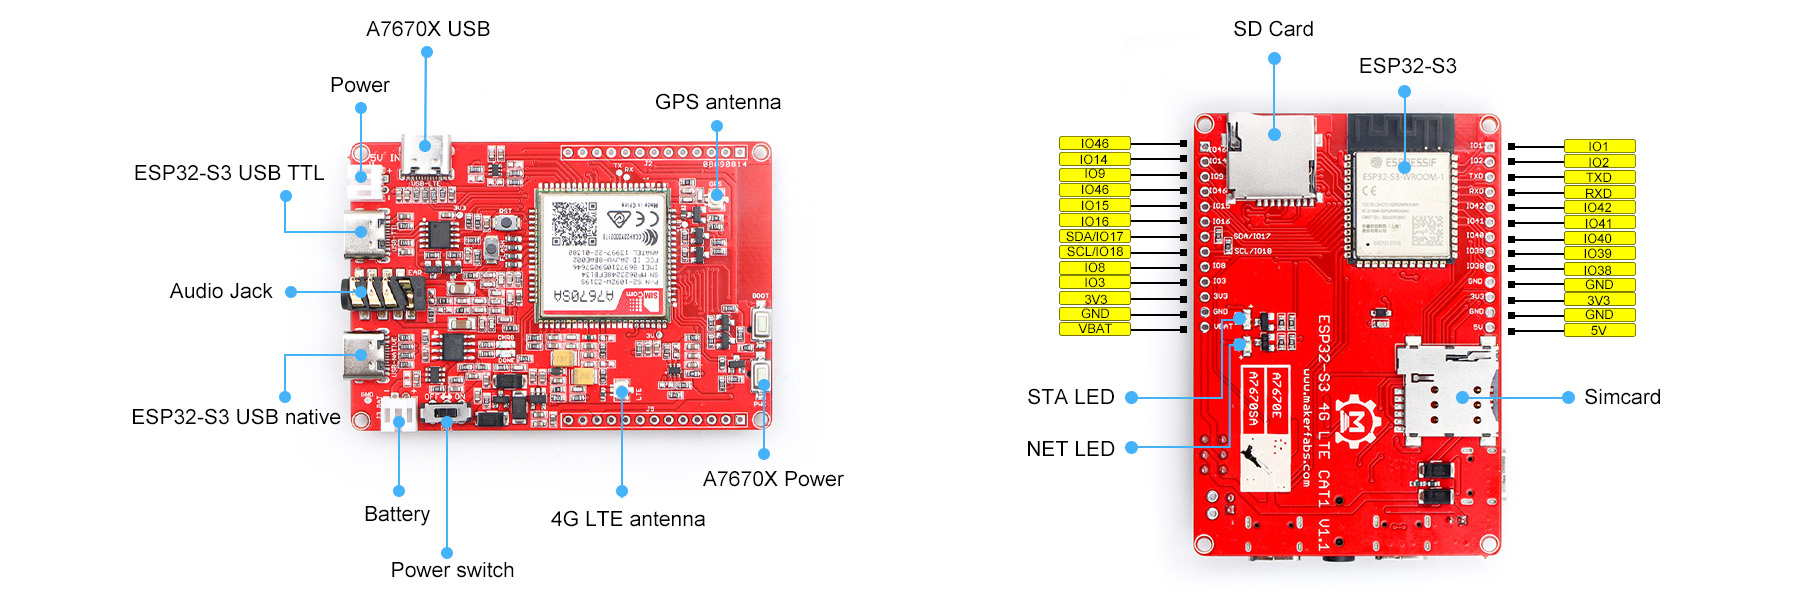
\includegraphics[width=\textwidth]{figures/makerfabs_a7670x_pinout.jpg}
\caption{Makerfabs ESP32-S3 4G LTE CAT1 A7670X board: manufacturer-labelled ports (left) and pinout (right) \cite{makerfabsa7670x}.}
\label{fig:makerfabs-pinout}
\end{figure}

\begin{figure}[htbp]
\centering
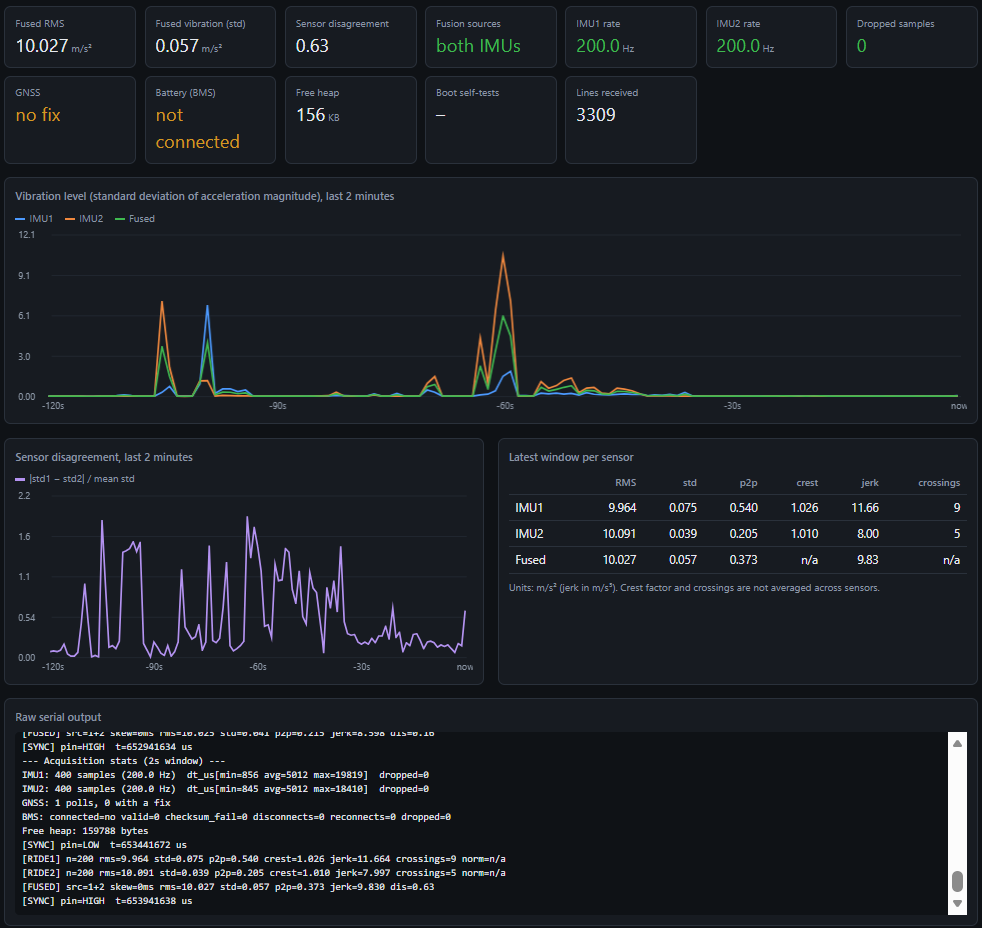
\includegraphics[width=0.85\textwidth]{figures/live_dashboard.png}
\caption{The live telemetry dashboard connected to the telemetry unit over USB during bench testing, showing both IMUs fused at 200\,Hz with no dropped samples and two hand disturbances in the vibration plot.}
\label{fig:live-dashboard}
\end{figure}

\begin{figure}[htbp]
\centering
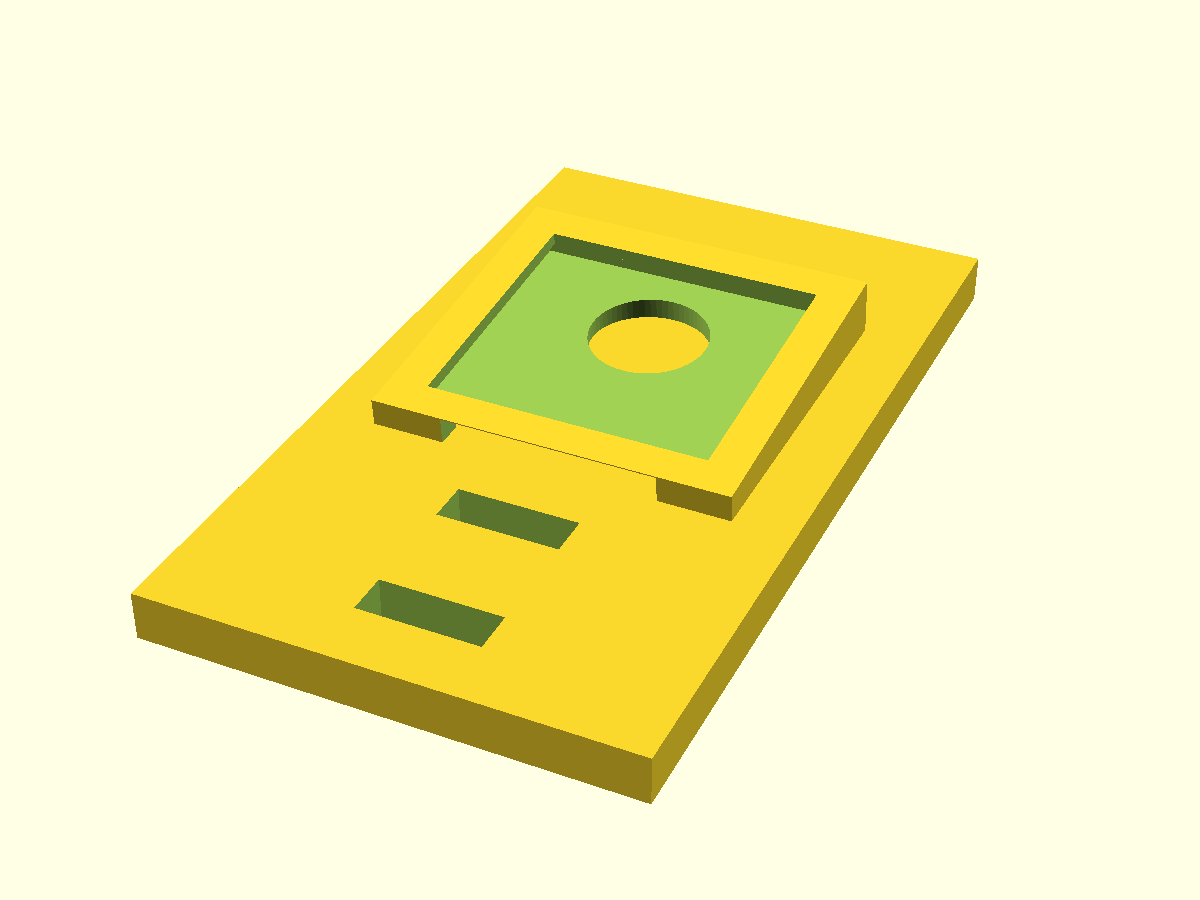
\includegraphics[width=0.6\textwidth]{figures/camera_mount_render.png}
\caption{Initial parametric camera bracket (OpenSCAD, full render), showing the corrected lens-retention lip and cable-routing slots. This design was not printed.}
\label{fig:camera-mount}
\end{figure}

\chapter{Test Evidence}
\label{app:evidence}

This appendix indexes the raw evidence behind the bench results reported in Chapter~\ref{chap:method}. Every item is the unedited output of the test it names and is kept in the project repository, under \texttt{Report/evidence/} or \texttt{BenchTest/logs/}; Table~\ref{tab:evidence-index} gives each file. Figure~\ref{fig:live-dashboard} in Appendix~\ref{app:figures} and Figure~\ref{fig:recorded-session} in Chapter~\ref{chap:method} belong to the same record.

\begin{longtable}{|p{1.7cm}|p{3.6cm}|p{5.2cm}|p{3.6cm}|}
\caption{Index of test evidence.}
\label{tab:evidence-index}\\
\hline
\textbf{Date} & \textbf{Test} & \textbf{Result shown} & \textbf{File} \\ \hline
\endfirsthead
\hline
\textbf{Date} & \textbf{Test} & \textbf{Result shown} & \textbf{File} \\ \hline
\endhead
25 Sep 2026 & Recorded bench session, telemetry unit, 150\,s from power-up & 200\,Hz on both IMUs with no dropped samples; 149 fused windows, all from both sensors; five of five fusion self-tests passed; acquisition gaps of 25 to 30\,ms every 12\,s & \texttt{BenchTest/logs/ 2026-09-25\_bench\_fusion\_shake.log} \\ \hline
25 Sep 2026 & The same log replayed through the bench console (Figure~\ref{fig:console-replay}) & Every subsystem's state at the end of the session, and the vibration and disagreement traces for the whole recording & \texttt{Report/evidence/ 2026-09-25\_bench\_console\_replay.png} \\ \hline
28 Sep 2026 & Hazard detector, first run on live camera frames & 430 frames in 60.1\,s (7.2\,fps); a person in view logged as ``motorcycle'', which exposed the label-offset fault & \texttt{Report/evidence/ 2026-09-28\_camera\_run1\_label\_bug.txt} \\ \hline
28 Sep 2026 & Hazard detector after the label and colour fixes & 419 frames in 60.1\,s (7.0\,fps); person detected at confidence 0.50 to 0.73; 16 alert activations in 47\,s for one person in view, which led to clear-side hysteresis & \texttt{Report/evidence/ 2026-09-28\_camera\_run2\_after\_fixes.txt} \\ \hline
29 Sep 2026 & Firmware v0.5.0 on the telemetry unit: commands, flash-write stall test, MQTT reconnect & With logging on, 33 to 40\,ms gaps on both IMUs every 10\,s; with logging off, worst gap 5.9\,ms; no dropped samples; 47 MQTT publishes with no failures; reconnect in 0.4\,s & \texttt{BenchTest/logs/ 2026-09-29\_v050\_bench\_test.log} \\ \hline
29 Sep 2026 & GNSS outdoor fix on a rooftop, firmware v0.5.0, raw replies requested every 15\,s & 3D fix after 51\,s; 17-field reply with decimal degrees; old parser read satellite counts as the position; well-formed replies 2.4 and 5.5\,m from the phone's position; replies garbled by the competing query & \texttt{BenchTest/logs/ 2026-09-29\_gnss\_rooftop.log} \\ \hline
30 Sep 2026 & GNSS outdoor fix with the corrected parser (v0.5.2), raw replies printed by the firmware & 3D fix after 105\,s from a cold start; 23 to 25 satellites; over 104 fixes, median 2.7\,m and 95\% within 11.0\,m of the phone's position & \texttt{BenchTest/logs/ 2026-09-30\_gnss\_rooftop\_v052.log} \\ \hline
30 Sep 2026 & MQTT recovery from a 60\,s radio-off period (\texttt{AT+CFUN=4}, then \texttt{AT+CFUN=1}), v0.5.0 and v0.5.3 & Loss detected in 0.8 to 20.7\,s; retries at 30 and 60\,s; reconnect 36\,s after the radio returned in v0.5.0, about 5\,s in v0.5.3; no failed publishes afterwards & \texttt{BenchTest/logs/ 2026-09-30\_signal\_loss\_test.log}, \texttt{..\_v053.log} \\ \hline
30 Sep 2026 & Sync-pulse edges logged on the Pi (GPIO17, kernel timestamps), two 60\,s runs & Run 1: 16\,s burst of spurious edges, consistent with a disturbed contact; run 2: 121 edges, median interval 500.06\,ms, range 499.72 to 500.41\,ms & \texttt{BenchTest/logs/ 2026-09-30\_sync\_edges\_run1\_noisy.csv}, \texttt{..\_run2.csv} \ \hline
30 Sep 2026 & Camera detector latency on the Pi, three 60\,s runs (4 threads, 4 threads with live view, 1 thread) & Median 102, 105 and 186\,ms from sensor readout to result; 19.5, 17.3 and 7.0 frames per second; no throttling & \texttt{BenchTest/logs/ 2026-09-30\_c4\_latency/} \ \hline
\end{longtable}

\begin{figure}[htbp]
\centering
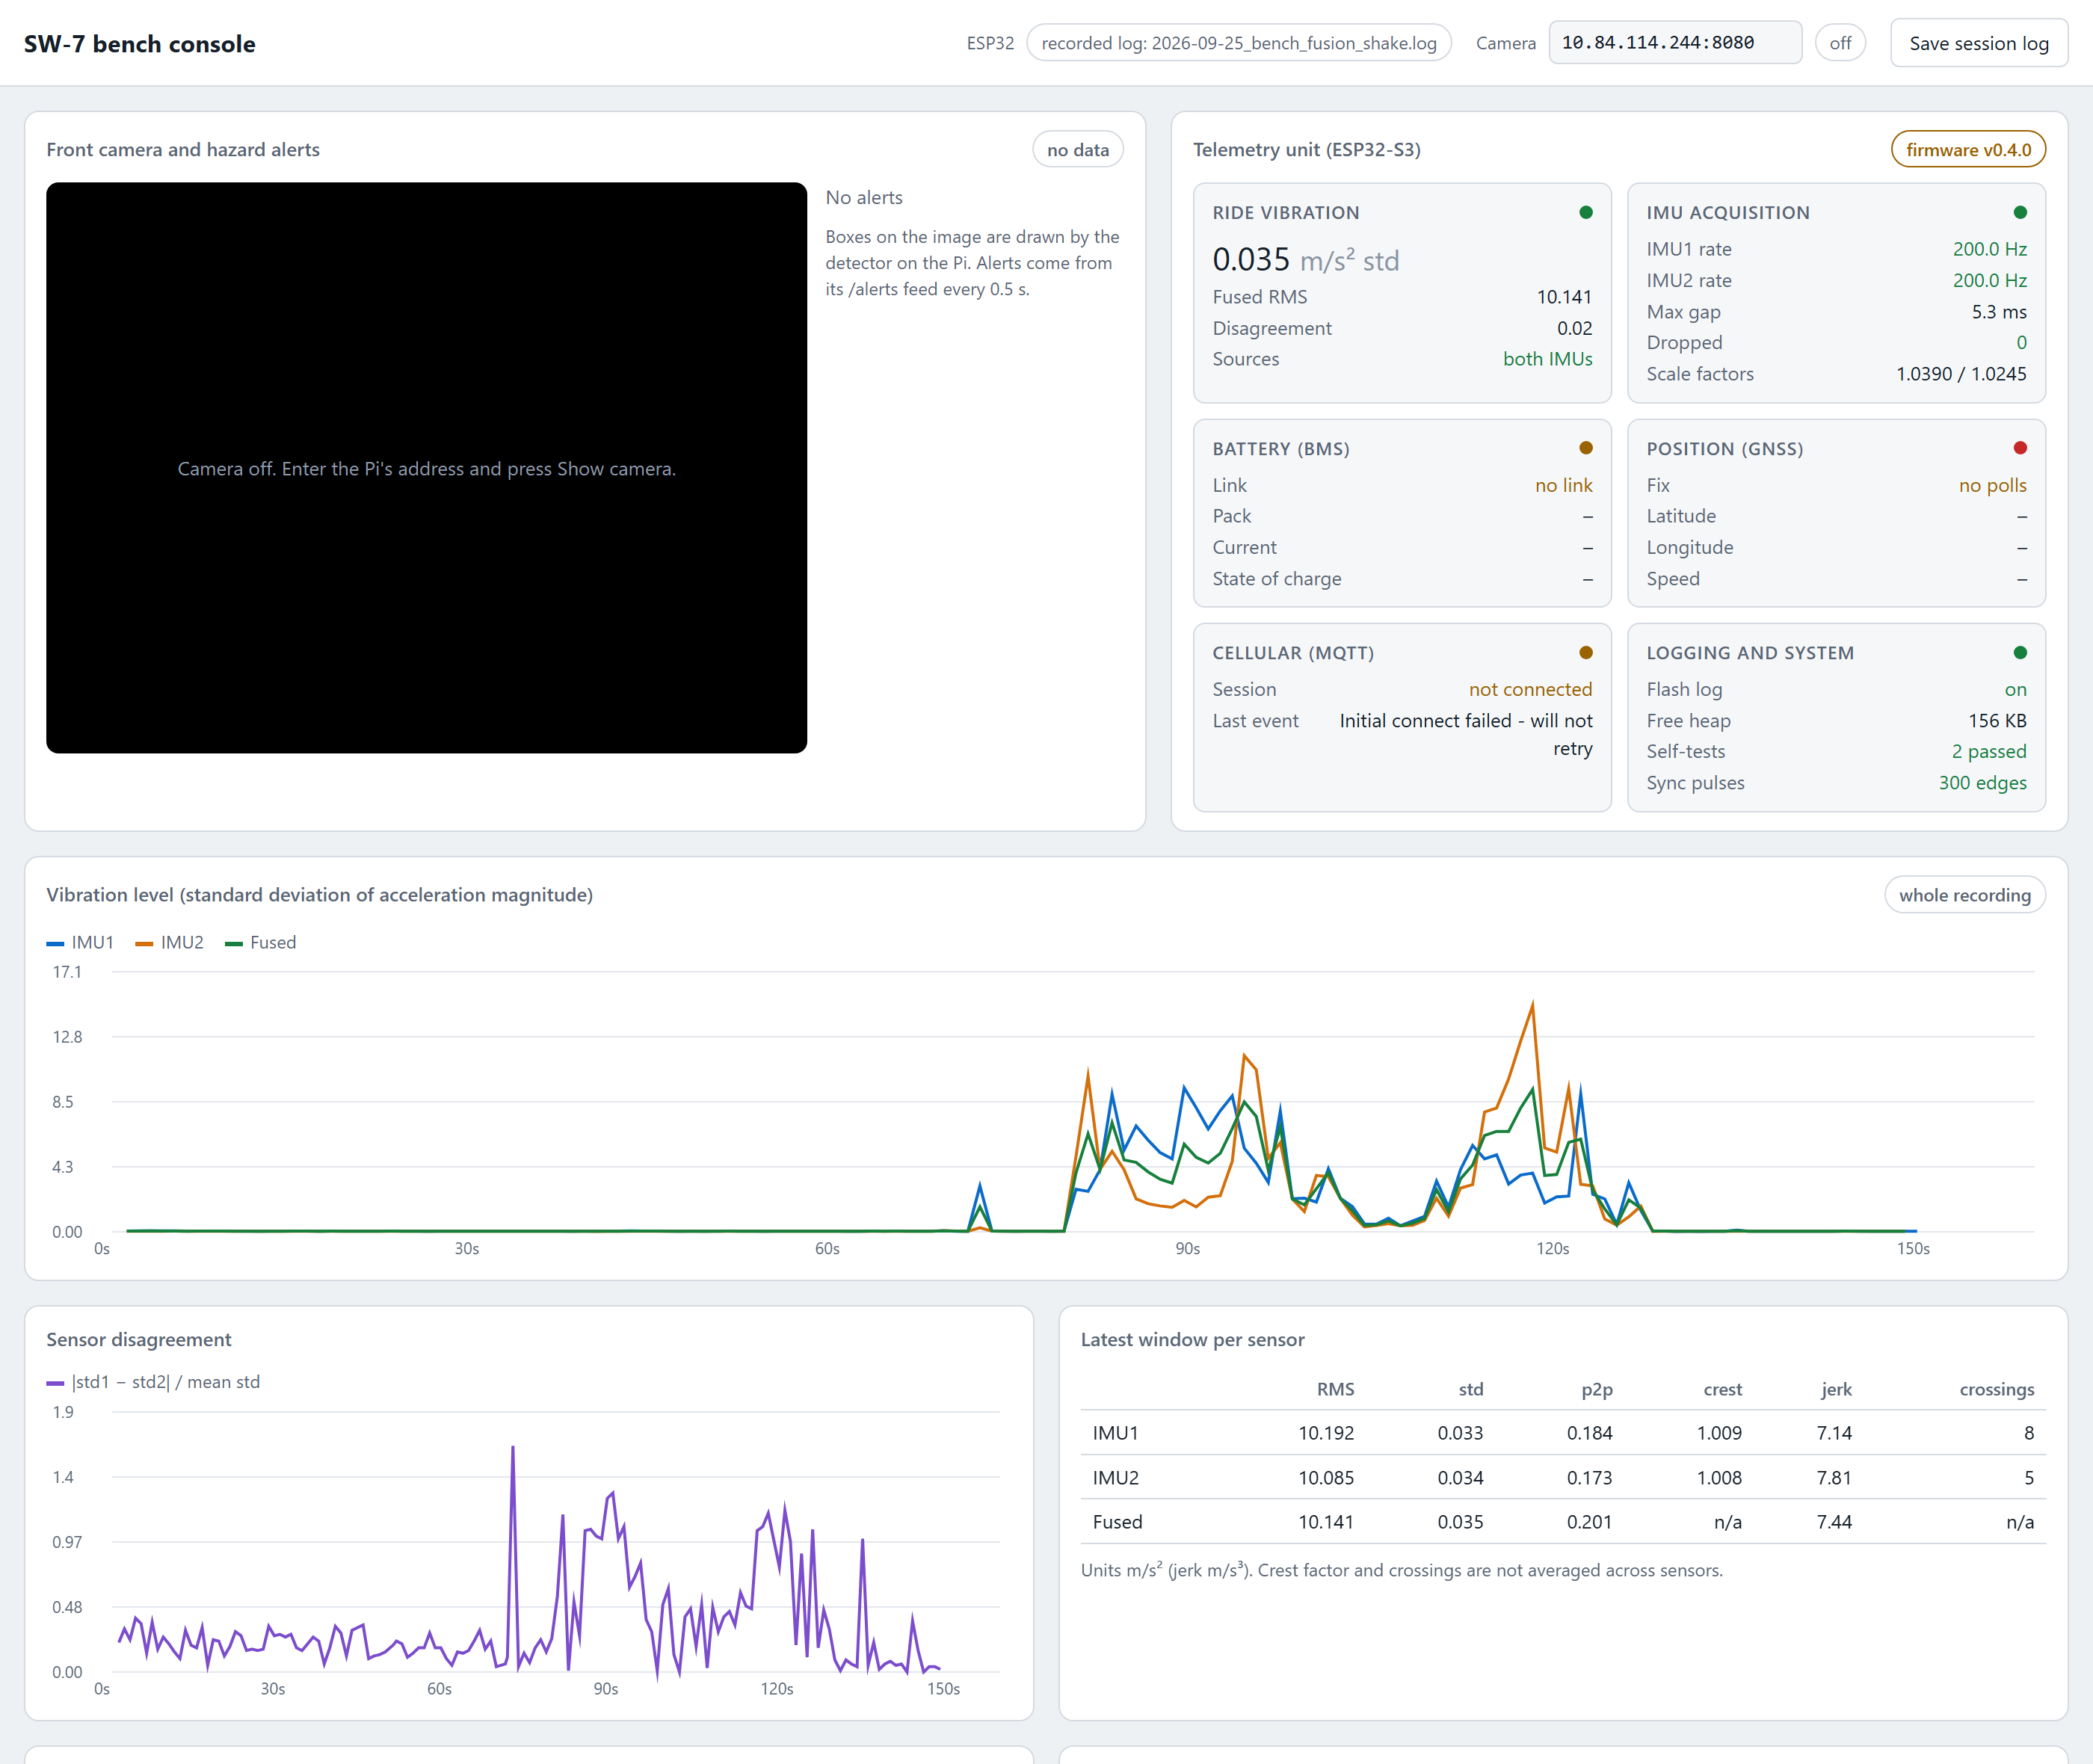
\includegraphics[width=\textwidth]{evidence/2026-09-25_bench_console_replay.png}
\caption{The recorded bench session of 25 September 2026 replayed through the bench console, which parses the telemetry unit's serial output. Only recorded data is shown; the camera panel is off because the camera was not part of this session.}
\label{fig:console-replay}
\end{figure}

The two detector runs end with the following lines, copied from the Raspberry Pi terminal. Before the fixes, every alert carried the wrong class:

\begin{verbatim}
Stopped. 430 frames in 60.1s (7.2 fps average).
{"class": "motorcycle", "distance_band": "immediate", "confidence": 0.66,
 "timestamp": "2026-09-28T11:58:32", "alert_status": "active"}
\end{verbatim}

After the fixes, the class is correct, and the log shows the alert clearing and re-activating within a few seconds while the same person stayed in view:

\begin{verbatim}
[14:31:28] person band=immediate conf=0.59 streak=3/3
  -> ALERT logged: person (immediate)
Stopped. 419 frames in 60.1s (7.0 fps average).
{"class": "person", "distance_band": "immediate", "confidence": 0.59,
 "timestamp": "2026-09-28T14:31:28", "alert_status": "active"}
{"class": "person", "distance_band": null, "confidence": 0.0,
 "timestamp": "2026-09-28T14:31:30", "alert_status": "cleared"}
{"class": "person", "distance_band": "immediate", "confidence": 0.59,
 "timestamp": "2026-09-28T14:31:31", "alert_status": "active"}
\end{verbatim}

}
\end{document}
